\documentclass[a4paper,11pt]{article}
\usepackage[utf8]{inputenc}
\usepackage{listings}
\usepackage{mathtools}
\usepackage{color}
\usepackage{amssymb}
\usepackage{tikz}
\usepackage{tkz-graph}
\usepackage{caption}
\usetikzlibrary{fit,arrows}
 \usepackage{booktabs}
 \usepackage{tabularx}
 \usepackage{mathtools}
% \usepackage{glossaries}



\usepackage{algorithmic}
%\usepackage{algorithm}
%\usepackage{algorithm2e}
\usepackage[linesnumbered, ruled,lined,boxed,commentsnumbered]{algorithm2e}

%opening

\newcommand{\method}[1]{\lstinline[basicstyle=\sffamily]{#1}}
\newcommand{\interface}[1]{\lstinline[basicstyle=\sffamily]{#1}}


\title{A General Purpose Local Search Solver}


\begin{document}

\maketitle
%\newpage
%\begin{abstract}

%\end{abstract}
%\newpage
\tableofcontents
%\listoffigures
%\listoftables
%\printglossary
%\makeglossary
\newpage
\section{Introduction}
 The field of optimization can be split into several subfields depending on the nature of the decision variables 
(continuous, discrete) and the structure of the problem (linear, non linear, combinatorial, convex, non 
convex). The main focus of this thesis is discrete optimization both linear and non linear. 
Several solvers are available for discrete optimization. The mixed integer linear programming (MILP) approach has 
solvers such as \emph{GLPK}, \emph{Gurobi} and \emph{CPLEX}. There are also constraint programming (CP) solvers, such 
as \emph{Gecode}. All these solvers solve the problem exactly, but for some problems thit is not always possible due to 
the computational cost. Another approach is to use local search and find a good solution fast by making a trade off 
between speed and solution quality. \medskip \\ 
There exists a vast literature about how to make good local search solvers for specific problems.
However, only a few attempts have been made to use local search for general purpose solvers like 
mathematical programming and constraint programming. \emph{Comet} was a successful CP based solver and that allowed to 
use local search to find a good solution fast but the project is now abandoned.  \\ 
\emph{OscaR} is another CP based solver that uses local search to find a good solution. 
\boste{OscaR}
% Currently LocalSolver is a commercial 
% product that combines a local search solver with a problem modeling language. It can be used to solve mathematical, 
% constraint, continuous, and non linear programming. \medskip \\
\boste{Overall made}
In this project, a general heuristic solver based on local search has been developed. It uses Gecode to find 
an initial solution and uses local search trying to improve the solution. It can solve problems formulated as binary 
programming problems but can be extended to solve a wider range of problems. Ideas for structuring the framework are 
drawn from Comet, OscaR, and Gecode. \medskip \\
\boste{More specific}
Beside the basic components of local search several elements have been studied to see their effect on the solution.
 One of these elements is preprocessing, with the help from Gecode, that can reduce the size of the search space before 
the local search is started. Other elements that have be studied are invariants and a directed acyclic graphs to 
represent efficiently the dependencies between the variables and invariants. The choice of neighborhoods and how to 
efficiently explore these neighborhoods have been considered. The quality of a solution is evaluated by a vector in 
lexicographic order instead of a single value. The lexicographic order is from a priority given to the constraints that 
will affect the local search. Finally, on top of the local search different combinations of neighborhoods, procedures, 
and metaheuristics has been tested. \medskip \\   
The framework has a solid base from which it can be extended to solve a wide range of problems by implementing 
different constraints and new neighborhoods. \medskip \\
The performance of the solver has been tested with the instances from the MIPLIB 2010 and compared to Gurobi.  



 
 
\section{Discrete Optimization}

  \subsection{Variables} 
  Models contains a set of $n$ variables $X = \{ x_1, x_2, \dots , x_n \} $. Each 
variable $x_i \in X$ has a \emph{domain} $D(x_i) \in D$ where $D$ is the cartisian produkt of n domains $D = 
 D_1 \times D_2 \times \dots\times D_n $ such that $x_i \in D_i$. The variables $x_i \in X$ of the models that will be 
discussed in this thesis all have their domain restricted to a finite discrete domain $D_i \subseteq \mathbb{Z}\ : \: 
\forall i$ \boste{should i declare a set $I = \{1,2,\dots , n\}$?}. The value of a variable $x$ is denoted $V(x)$ and 
we will denote integer variables as $y_i \in Y \subseteq X$.  % Written
  \subsection{Constraints}
  The variables will be restricted by $C$ that is a m-tuple of constraints $C= \langle 
c_1,c_2, \dots , c_m \rangle $. The set of variables to which the constraint $c_j$ applies is called its scope and 
is denoted $V(c_j)$ or ($X(c_j)$ and $Y(c_j)$ for the binary and integer variables respectivly). Each $c_j \in C$ is a 
pair $\langle R_{V(c_j)}, V(c_j) \rangle $ where $ R_{V(c_j)}$ is a subset of the 
cartesian product of the domains of the variables in $V(c_j)$ also called the relation on $c_j$. \\ 
The Constraint Satisfaction Problem (CSP) can then be defined as a triple $\mathbb{P} = \langle V,D,C \rangle$. A 
solution to the CSP $\mathbb{P}$ is a n-tuple $A = \langle a_1,a_2,\dots,a_n\rangle $ where $a_i \in 
D_i$. The solution is feasible if the projection of $A$ onto $V(c_j)$ is included in $R_{V(c_j)}$ for all 
$c_j \in C$.\\ 
The solution of interest could be all feasible solutions $sol(P)$, any feasible solution $S$ or if there 
exists a solution or not. \\ 
The CSP can be expanded to a Constraint Satisfaction Optimization Problem (CSOP) with an objective function $f(S)$ 
that evaluate the quality of the solution $S$. The task is then to find a solution $\hat{S}$ that gives minimum or 
maximum value of $f(\hat{S})$ depending on the requirements of the problem. \\ \\ 
While constraint programming often offers a wide selection of constraints to use, this thesis focus mostly on the 
constraint Linear that is defined by a left hand side, a relation and a 
right hand side, which is a constant bound $b$. The left hand side is a linear function of decision variables 
multiplied with their coefficient. The relation between left hand side and right hand side is restricted to be one of 
the six: less ($<$), less or equal ($\leq$), greater($>$), greater or equal($\geq$), equal ($=$), and disequal 
($\neq$). \boste{Ikke særlig pænt, men ved ikke hvordan jeg 
skal beskrive det ellers (Gecode har seks, MIP og IP har kun 3)}\\ 
A linear constraint $c$ can be described as: 
\begin{equation}
 \sum A(c) \cdot V(c) \lesseqgtr B_c
\end{equation}
The coefficients $A(c)$ are the coefficients of the variables in the scope of $c$. The decision variables $V(c)$ are 
the variables that $c$ applies to. The bound $B_c$ is the bound for the left hand side in constraint $c$. \\ 
MIP, IP and BP are restricted to use the linear constraint and the model is often written as: 
\begin{align}
 \text{Minimize } & \mathbf{c}^T\mathbf{x} \nonumber \\ 
 \text{Subject to } &\mathbf{Ax} \leq \mathbf{b} \nonumber\\
 &\mathbf{x} \in \mathbf{D}
\end{align}





%In order to define mixed integer programming and integer programming we need to define a function $f(X) = 
%\sum_{x_i \in X} 
%c_i x_i$ where $c_i \in E 


%We can reduce the CSP to 3-SAT by restricting the domain of the variables to zero and one and restrict the scope of 
%all constraints to exactly three. By that we can conclude that some CSP are NP-complete and not easy to solve.   % split it into constriants and CSP
  \subsection{Problem Formulation} % CSP-> CSOP
  A \emph{Constraint Satisfaction Problem} (CSP) is defined as a triple $\mathbb{P} = \langle X,D,C \rangle$. A 
\emph{candidate solution} to a CSP $\mathbb{P}$ is a vector of $n$ elements \\
%$\tau = (\tau_1,\tau_2,\dots,\tau_n) $ where $\tau_i \in D_i$. 
$\tau = (V(x_1), V(x_2), \dots , V(x_n))$ from the set of all candidate solutions $S$ called the \emph{search space}.  
% D_1 \times D_2 \times %\dots , D_n) $ where $\tau_i \in D_i$. 
Given a sequence $X' \subseteq X$ of variables $\tau[X']$ is called a restriction on $\tau$, ordered according to 
$X$. If the restriction $\tau[X(c_j)]$ matches a tuble of the constraint $c_j$ in extensional form the solution $\tau$ 
satisfies constriant $c_j$. If each constraint $c_j \in C$ is satisfied then the solution $\tau$ is a \emph{feasible 
solution} to the CSP $\mathbb{P}$. \\


  \subsection{Solutions}
  For a CSP the questions of interest could be to report all feasible solutions $sol(P) \subseteq S $, any feasible 
solution $\mathbf{\tau}\in sol(\mathbb{P})$ or if there exists a feasible solution $\mathbf{\tau}$ or not. \\
The CSP $\mathbb{P}$ can be expanded to a \emph{Constraint Optimization Problem} (COP) $\mathbb{P'}$ 
with an evaluation function $f(\mathbf{\tau}) \rightarrow \mathbb{R}$ that evaluates the quality of the solution 
$\mathbf{\tau}$, $\mathbb{P'} = \langle X,D,C,f) \rangle$.  In the COP the task is then to find a feasible solution 
$\hat{\mathbf{\tau}}$ in $S$ such that $f(\hat{\mathbf{\tau}}) \leq f(\mathbf{\tau})$ for all feasible solutions $\tau$ 
of $\mathbb{P}$ if it is a minimization problem. \\ 
  
  
\newpage  
\section{General Purpose Solution Methods}  
  
  \subsection{Binary- and Integer Linear Programming} % In general, talk about Gurobi, Scip, Cplex after
  Binary- and integer linear programming can be used to model a wide range of problems by posting linear constraints and 
using and a linear objective function. A linear integer program can be writing on the form: 
\begin{align}
 \text{Minimize }\; &z =  \mathbf{c}^T\mathbf{x} \\ 
 \text{subject to } \; & A\mathbf{x} \leq \mathbf{b} \\ 
 & \mathbf{x} \in \mathbb{Z}^n
\end{align}
Here $A$ is a $n \times m$ matrix of coefficients, $\mathbf{b} \in \mathbb{R}^m$, $z$ is the value of the objective 
function and $\mathbf{c} \in \mathbb{R}^n$. The first line is the objective function and can easily be transformed to a 
maximization problem by multiplying by $-1$. The relation in line 2 can be a mix of $\{\leq,=,\geq\}$ but $\geq$ can 
be transformed to $\leq$ by multiplying both side of the constraint by $-1$.  \\ 
A solution is an assignment of values to all variables $\mathbf{x}$ and a solution is said to be feasible if all 
constraints are satisfied. The set of feasible solutions consist of integer point in a $n$ dimensional space and the 
point that minimize the objective function is said to be the optimal solution. \\
Solving a general integer program or binary program is a NP-hard problem and several techniques are developed for 
solving them. The techniques can be i.e. branch and bound, cutting plane and branch and cut and usually by
relaxing the integer constraint to solve an auxiliary linear problem \cite[p. 30]{ilp}. The linear problem can be 
formulated as the integer linear problem where variables can take real values. The linear formulation can be 
transformed to standard form by introducing auxiliary variables and then solved using the simplex method. The relaxed 
problem can be used as a lower- or upper bound depending on whether the problem is a minimization or maximization 
problem. \boste{Jeg ved ikke om jeg skal uddybe det mere, når jeg kun beskæftiger mig med BP/IP} \\ 
There exist several solver for (integer) linear programming problems such as Cplex, Gurobi, GLPK and Scip. 
  
  \subsection{Constraint Programming}
  Constraint programming involves defining variables and constraints like ILP but often a wide range of constraints can 
be used. Constraint programming is declarative programming that is the program describe the desired result 
and not the commands or steps to reach it, just like ILP. Constraint programming uses some interface either a 
programming language or a framework that have procedures implement to solve the problem according to the constraints 
posted. The language or framework may provides global constraint that can be used to formulate the problem. An example 
of a global constraint is the {\sffamily{alldifferent(\textbf{x})}} constraint that specify the variables \textbf{x} 
must have pairwise distinct values.  \\ 
Two important aspects of solving a CSP are inference and search. \emph{Inference} is adding constraints to the CSP that 
does not eliminate any feasible solution but might make it easier to solve the CSP \cite[p.301]{CPbog}. 
Local constraint propagation is an example of inference when dealing with variables with finite domain and can be used 
to eliminate large subspaces of the search space $S$. Propagation can be restricting domains of variables, called 
filtering, or combinations of values to variables, based on the constraint doing propagation \cite[p. 169]{CPbog}. 
Propagation can be done when a constraint is created by eliminating values from the domain of variables. I.e. by 
doing propagation on the constraint $x_1 + x_2 \leq 2$ where $x_1,x_2 \in \mathbf{Z}^+$ we can reduce the domain of the 
variables to $\{0,1,2\}$. If we set $x_1 =1$ we can again do propagation and reduce the domain of $x_2$ to $\{0,1\}$. 
\\ 
Search strategies explores possible assignments of variables and an exhaustive search would be a combination of all 
possible assignments of values to the variables. When combining propagation and search strategies the search space can 
be examined exhaustively and large subspaces can be pruned by propagation. \\ 
COP
    \subsubsection{Implicit Constraints}
    \emph{Implicit constrains} are constraints that\boste{, once satisfied,} always stay satisfied during local search. 
Each neighborhood operations is made in a way that implicit constraints are kept satisfied. 
    \subsubsection{Gecode}
    Gecode (generic constraint development environment) is a constraint programming solver implemented in C++ and 
offer a wide range of modeling features. Gecode offers more than 70 constraints from the ``Global Constraint Catalog'' 
\cite{url_globalCons} that can be applied to boolean, integer, set and float variables. \boste{Muligvis Gecode 
architecture billede} \\ 
A model created for Gecode is created by inheriting the space class. Space is is a basic layer in Gecode that a user 
can build the model on. To Create variables or post constraints the user need to specify the space they should be 
created in. When variables are created in a space, views are created and associated with the variables. 
Views are not used in modeling but are used to know when propagation should be made on a constraint.  When posting 
constraints in a space, Gecode creates propagators and these propagators can subscribe to the views of the variables 
in the constraint. When variables changes domain the corresponding view tell its subscribes that the variables domain 
has changed. For some constraint the user has the option to choose the propagator based on a consistency level. 
The cost of different consistency level varies from linear in the number of variables to exponential \cite[p.57]{MPG:M}. 
\\
To solve a problem Gecode needs guidance when searching and that is done by a branch function. Once a problem has been 
formulated, the user must define on which variables and how branching is done. Just like variables and constraints are 
posted in a space the branch order is also posted on the space. The choices in branching for a set of variables are 
which of those variables to branch on first and what values to branch on. One can post several branch methods and they 
are treated in the order they are posted. Once all variables have been branched in one branch function it continues 
with the  If no branch strategy is chosen for a variable then branching is not done on that variable. \\ 
To start the search a search engine must be chosen and Gecode offers two, a depth first search engine and a branch and 
bound engine. Search engines have an option class in which several options can be set \cite[p.157]{MPG:M}. \\ 
When searching for a solution in a space, the search can be illustrated as a binary tree where the edges are 
branch choices for a variable and the vertices are the space created because of those choices. If it reaches a point 
where no solution is possible it stop branches from that vertex and the space is said to be failed. While searching for 
solution sometimes, based on a search parameter from the option given, Gecode clones the spaces. When Gecode 
reaches a failed space, instead of starting from scratch and recompute all way to down to the previous vertex, it 
uses the closest clone to backtrack to that space. \\
  \subsection{Heuristics and Local Search}
  In contrast to integer programming and constraint programming, local search does not do an exhaustive 
search for a solution. Local search is based on making small changes to the current solution and 
see if it can improve and sacrifices the optimality guaranty for performance. \\ 
To create a model for local search a set of variables and a set constraints for the variables needs to be defined. The 
constraints are implicit constraints and some might need to be relaxed to soft constraints. The variables and implicit 
constraints define the candidate solution and hence the search space $S$.

     \subsubsection{Basic Aspects of Local Search}
    There are several important aspects of local search and the most basic will be covered here. \\The evaluation function 
$f(\tau)$ evaluate the quality of the candidate solution. 
The \emph{step function} that defines the candidate solutions close to a given candidate solution $\tau$. By applying 
the step function once to candidate solution $\tau$ a new candidate solution $\tau'$ is obtained. Going from one to 
solution to another with the step function is called a \emph{step}. Several solution might be explored before making a 
step and using a \emph{neighborhood operation} defines by the step function.  Local search uses a neighborhood function 
$N(\tau)$ that for each solution $\tau \in \S$ specify a subset of solutions $N(\tau) = \Tau$. The solutions $N(\tau)$ 
is called the neighborhood of $\tau$ and are the set of solution that can obtained by making one step. The cardinality 
of $N(\tau)$ is called the neighborhood size of $\tau$ and depends on the step function. The neighborhood function $N$ 
is symmetric if, $\tau' \subseteq N(\tau)$ if and only if $\tau \subseteq N(\tau')$ for all pairs of $\tau$ and $\tau'$. 
In a problem with $n$ binary variables the step function could be to change the value of a single variable, a flip.  
This can be done on all variable hence the neighborhood size of a candidate solution would be $n$. \\ 
It might be expensive to use the evaluation function to evaluate each solutions, instead a \emph{delta evaluation 
function} $\delta(\tau)$ can be used. The evaluation function recomputes the quality of a solution even if only a few 
variables changes value. The delta evaluation function only computes how much the evaluation function will change by 
going from one solution $\tau$ to another solution $\tau'$, hence $\delta(\tau) = f(\tau')-f(\tau)$. \\
The search space combined with the neighborhood function can be illustrated as a graph $G = (V,E)$. The set $V$ is a 
set of vertices each representing a candidate solutions of $S$ and $E$ is a set of edges connecting a vertex v, 
representing the solution $\tau$, with the vertices representing $N(\tau)$. The graph $G$ is called the neighborhood 
graph and local search does a walk through the neighborhood graph when searching for a solution. \cite[p. 3-5]{lsbog} 
\\ 
Local search needs a \emph{termination criteria} that determines when the search should stop. Sometimes we know what 
an optimal is, i.e. the SAT problem, once we find a feasible solution we can stop. In other cases an optimal solution 
may not be know, several combinatorial problems are not solved to optimality. The termination function can i.e. be based 
on a time limit, number of steps made, or when a locally optimal solution is found. A locally optimal solution for 
a minimization problem is a solution $\hat{\tau}$, such that for each feasible solution $\tau \in N(\hat{\tau})$ 
$f(\hat{\tau}) \leq f(\tau)$. \\

    \subsubsection{Local Search Algorithms}
    When a local search algorithm makes a neighborhood operation from a current solution to a new solution we say it 
commits the neighborhood operation. One of the basic local search algorithms is the \emph{iterative 
improvement} with different pivot rules. Iterative improvement explores the neighborhood of the current solution or a 
subset of the neighborhood and uses the delta evaluation function to determine which of the neighborhood operations 
to commit. \\ 
Two basic pivoting rules for iterative improvement are \emph{best improvement} and \emph{first improvement}. Best 
improvement examines all solutions in the neighborhood of the current solution with delta evaluation function and 
chooses the solution that gives the best improvement, if any. First improvement examine the solutions in the 
neighborhood and commits the first neighborhood operation that gives an improvement, if any. Iterative 
improvement is repeated until no improving solution exists. \\ 
Several heuristics can be applied to the algorithms for instance by choosing a subset of the neighborhood to examine at 
random when using best improvement or allowing a number of consecutive sidewalks. A sidewalk is going from a solution 
$\tau$ to a neighbor solution $\tau'$ where $\delta(\tau') = 0$. First improvement can be modified to \emph{random 
improvement} that chooses an improving solution with a probability $p$ or looks for the next improving solution with 
probability $1-p$. \\ 
Another basic local search algorithm is the \emph{random walk}. Random walk commits a neighborhood operation chosen 
uniformly random and repeats that for number of iterations. This might lead to a worse solution and/or infeasible 
solution and it is usually combined with other heuristics or local search algorithms. \\
Before local search can be done an initial assignment to the variables is needed and an initialization function is 
used for this also called a construction heuristic.  \label{sub_lsalg}
    \subsubsection{Construction Heuristics}
    A construction heuristics is used to find an initial candidate solution to a given instance. One of the main things to 
consider when creating a construction heuristic algorithm is the balance between quality of the solution and time 
complexity of the algorithm. The extreme case would be to solve the given instance with a construction heuristic but 
then the main point of local search is lost, which is finding a high quality solution fast. \\ 
The first thing to consider when creating a construction heuristic is whether it has to find a feasible solution or it 
is allowed to find an infeasible solution. The choice depends on how the local search is designed, whether it can reach 
infeasible solutions or not. \\ 
An example of a simple construction heuristic is creating a random candidate solution. For each variable a value 
between its lower and upper bound is chosen uniformly at random. This is a fast construction heuristic $O(n)$ but 
cannot give any guarantee of the quality. Examples of other construction heuristics could be greedy heuristics like 
first fit or best fit. \\ 
Construction heuristics can be tailored to a specific problem type to find a good initial solution depending on 
the problem. It can be beneficial to introduce randomness in the algorithm and rerun it a couple of times to get a 
better initial solution.
    \subsubsection{Metaheuristics}
    Metaheuristics defines how the search space should be explored, whereas local search algorithms focus more on 
the neighborhood of the solution. Iterative improvement often find a local optimum quickly, depending on the size of 
the neighborhood. Usually only a small fraction of local optima are close to optimality and they can be a poor quality 
solution \cite[p.135]{lsbog}. Metaheuristics are used to get out of local optima to search different parts of the 
search space. \\
A simple metaheuristic is \emph{iterative local search} that remembers the best solution found so far and uses two 
local search algorithms, random walk and iterative improvement. It uses iterative improvement 
to find a local optima and compare it to the best solution so far. Then uses random walk for some iterations to escape 
the local optima. These two algorithms are repeated until the termination criteria is reached. \\ 
Another metaheuristic is \emph{tabu search} that implements an iterative improvement with a modified best improvement 
pivoting rule. It chooses the neighborhood operation that will leads to the best solution in the neighborhood, but not 
necessarily a better solution. In addition to the modification of the pivot rule it implements a tabu list $T$ that 
keeps track of the last $t$ solution. The solutions in the tabu list are not considered when looking for the next 
solution. It might be very memory expensive to keep track of the last $t$ solutions. An alternative way of implementing 
the tabu list is to keep track of the last $t$ neighborhood operations and forbid the reverse neighborhood operations. 
This is more restrictive since the reverse neighborhood operations might not lead to a solution visited within 
the last $t$ iterations. To compensate for this an \emph{aspiration criteria} can be implemented. Aspiration criteria 
is 
a set of rules that can overrule the tabu list \cite[p.139-140]{lsbog}. A common aspiration criteria is to ignore the 
tabu list if the neighborhood operation leads to the best solution found so far. \\
Several other metaheuristics exist such as variable neighborhood search and very large scale neighborhood 
search. Variable neighborhood search uses different neighborhood functions, hence different neighborhoods. Very large 
scale neighborhood search changes many variables in each neighborhood operation, which gives a very large neighborhood, 
but might need fewer iterations to find a good quality solution. 
    \subsubsection{Creating a Model for Local Search}
    When creating a model for local search there is several things to consider, most important things to consider are what 
the variables should represent and what constraint should be imposed on them. The choice of variables and constraints 
together with the step function should be such that the delta evaluation can be calculated fast, preferably $O(1)$. The 
step function should be chosen such that the search space can be explored efficiently. One thing to consider is whether 
allowing candidate solution that are infeasible or not, once a feasible solution is found.  
  \subsection{Constraint Based Local Search}
  \emph{Constraint based local search} (CBLS) is trying to combine the concept of constraint programming and local 
search. Constraint programming gives a natural way of describing a problem and can reuse the global constraint, 
propagators, and search strategies. Local search has concepts such as moves, neighborhood, and metaheuristics that have 
specific implementations for each problem type. Local search offers high quality solution within a relatively short time 
limit. \\ 
The idea of a CBLS framework is to offer global constraint to formulate the problem while local search algorithms are 
used to solve the model. The user can focus on modeling their problem instead of creating and optimizing 
algorithms to solve it. This gives the reusability and formulation power of constraint programming while having the 
performance of local search.   \\ 
To increase efficintcy of local search, new data structures are introduced such as Invariants and oneway constraints. 
    \subsubsection{Invariants and Oneway Constraints}
    Invariants are variables, which value is purely determined by other variables. The variable defined is not necessarily 
one of the variable currently in the system but it can be a new auxiliary variable which value is of interest.  
The invariants all have generic methods that needs to be defined for the different types of invariants. One of these 
methods is for instance \method{getCurrentValue()} that return the value of the invariant. If a variable $v$ 
changes value then the invariants that are defined by $v$ needs to update their current value. This is done 
through the \method{addChange(arguments)} method, \method{calculateDeltaValue()}, and  \method{updateValue()}. They 
informs the invariant something is changed, calculates the change in value and updates the current value respectively. 
Since invariants can be defined by variables that are invariants themselves this can leads to a series of 
updates. Invariants and constraints can built as a directed graph without cycles in 
order to avoid looking at an invariant multiple times when a change is made to a variable. The construction of that 
graph is described in section \ref{updategraph}. \\ 
An example of an invariant is the \method{Sum} invariant that defines an auxiliary variable. The 
\method{Sum} invariant consist of a coefficient set $C$, variable set $V$ and it can have a constant $b$ added. For 
a \method{Sum} invariant $S$ the value is defined as: \\
\begin{equation}
 S = b+ \sum_{\substack{i \in I_S}}  c_i x_i  
\end{equation}



%which value is defined by the sum of the variables and invariant  times their coefficient. 
%Invariants are used to create auxiliary variables based on other variables and/or invariants. 
    \subsubsection{Soft Constraints}
    \emph{Soft constraints} are constraints that the local search should try to satisfy when making neigborhood operations. 
If a soft constraint is not satisfied we say it is violated and it contributes to the evaluation function. There are 
different ways of measuring the violation in a constraint. One way is a binary value, zero for not violated and one 
for violated. Another way is to use \emph{violation degree}, a measurement of how violated a constraint is, by a 
function depending on the constraint. I.e. for the \textbf{alldifferent(X)} constraint, that is all variables \textbf{X} 
must have pairwise distinct values, it can be the number of variables with the same value as another variable. \\ 


    \subsubsection{Evaluating Solutions}
    There are different ways of measuring the quality of an solution. For a CSP a feasible solution needs to be found but 
there is not distinguished between feasible solutions.  \\
In a COP the feasible solutions are compared by an objective function that gives the feasible solution a measurement 
of quality. \\ 
There are different ways of differentiating infeasible solution from other solutions, feasible or infeasible. The 
evaluation function is a combination of the objective function and the violated constraints. Each constraint can be 
given a weight and together with the violation degree it contribute to the evaluation function. I.e. a constraint has 
weight ten and a violation degree of three it then contribute 30 to the evaluation function. In this way the search 
priorities to satisfy certain constraints more than other. This method can have the negative effect that it might 
priorities to have all constraint with violation degree over one constraint with very high violation degree. \\ 
Another way it to use a priority for each constraint as a lexicographic ordering, rather satisfy a constraint with high 
priority than any number of constraints with lower priority. 
  %\subsection{Evaluation Function}
  %\input{objFunc}
    \subsubsection{Comet}
    %

% Figur om opbygning af comet som i bogen
Comet is an object oriented programming language that uses the modeling language of constraint programming and uses a 
general purpose local search solver. Comet is now an abandoned project, but the architecture used is still of interest. 
The core of the framework are the variables and invariants.
\medskip \\
One layer above the invariants are the differentiable objects that can use the invariants and variables. 
Both constraints and objectives are implemented as differentiable objects. They are called differentiable 
because it is possible to compute how the change of a variable value will affect the differentiable object's values. 
All constraints are implemented using the same interface, which means that all constraint have some methods in common. 
This is especially useful when combining multiple constraints in a constraint system. The constraints can be combined in 
a constraint system that then uses the method from the individual constraints to calculated its own methods. Just like 
the \interface{constraint} interface there exists an \interface{objective} interface. \medskip \\ 
The next layer is where the user models their problem and use the objects mentioned above. Several search procedures 
are implemented. The benefit of this architecture is that the user can focus on modeling the problem 
efficiently on a high level and thereby avoid small implementation mistakes. Using constraint programming inspired 
structure gives the benefit of brief, but very descriptive code. \\ 
The idea of structuring the constraint and invariant as interface is also used in this framework. 



%The core of framework is the incremental store that contains various incremental objects fx. incremental variables. 
%Invariants, also called one-way constraints, are expressions that are defined by incremental variables and a relation 
%of those. An incremental variable $v$ can for instance be expressed as a sum of other variables. The variable $v$ will 
%automatically be updated if one of the other variables changes value. The order in which the invariants are updated 
%can be implemented to achieve higher performance.  
    \subsubsection{OscaR}
    
  
%\section{Modeling Constraint Based Local Search}
  %\boste{Tror ikke det er så sammenhængende, mangler en mere blød overgang.}
  %\subsection{Types of Modeling \boste{not sure this should be here}}
  %%Section
The choice of modeling approach should depend on the nature of the problem. Constraint programming (CP) uses 
constraints to formulate a constraint satisfaction problem (CSP) and often provides short and natural way to 
describe a problem. Constraint programming try to find feasible solutions to a CSP hence it does not 
differentiate the solutions that might exist. One can work around that by creating a function that evaluates a 
solution by a value. Then add the constraint that the function must give a better value than last time. \\ 
\boste{Jeg ved ikke om jeg skal definere IP her eller tidligere (og hvor meget der skal skrive) } \\ 
Mixed integer programming (MIP) and Integer programming (IP) are more restricted in the choice of constraints. They can 
only use linear constraints hence the models often tend to be longer in order to formulate a problem. Unlike 
constraint programming both mixed integer programming and integer programming has an objective function that rates the 
quality of a solution. Binary programming (BP) models the same way as MIP and IP but restricts the variables from 
integer to binary. \\





    
 
%\section{Local Search}
%  \input{local}
%\section{Previous Work}
 % \subsection{Comet}
  %

% Figur om opbygning af comet som i bogen
Comet is an object oriented programming language that uses the modeling language of constraint programming and uses a 
general purpose local search solver. Comet is now an abandoned project, but the architecture used is still of interest. 
The core of the framework are the variables and invariants.
\medskip \\
One layer above the invariants are the differentiable objects that can use the invariants and variables. 
Both constraints and objectives are implemented as differentiable objects. They are called differentiable 
because it is possible to compute how the change of a variable value will affect the differentiable object's values. 
All constraints are implemented using the same interface, which means that all constraint have some methods in common. 
This is especially useful when combining multiple constraints in a constraint system. The constraints can be combined in 
a constraint system that then uses the method from the individual constraints to calculated its own methods. Just like 
the \interface{constraint} interface there exists an \interface{objective} interface. \medskip \\ 
The next layer is where the user models their problem and use the objects mentioned above. Several search procedures 
are implemented. The benefit of this architecture is that the user can focus on modeling the problem 
efficiently on a high level and thereby avoid small implementation mistakes. Using constraint programming inspired 
structure gives the benefit of brief, but very descriptive code. \\ 
The idea of structuring the constraint and invariant as interface is also used in this framework. 



%The core of framework is the incremental store that contains various incremental objects fx. incremental variables. 
%Invariants, also called one-way constraints, are expressions that are defined by incremental variables and a relation 
%of those. An incremental variable $v$ can for instance be expressed as a sum of other variables. The variable $v$ will 
%automatically be updated if one of the other variables changes value. The order in which the invariants are updated 
%can be implemented to achieve higher performance.  
  %\subsection{Gecode}
  %\subsection{LocalSolver}
%\subsection{Structure of this CBLS \boste{Differences from oscar and comet.}}
\newpage
\section{Architectural Overview}  
  This section gives an overview of the key components of the solver. The figure \ref{fig_architec} gives an overview 
of the most basic classes and the classes they have ponters to (access to). \\
\begin{figure}[!b]
\includegraphics[width=\linewidth]{architectureTest}\caption{Overview of what the classes contains pointers to} 
\label{fig_architec}
\end{figure}
The two engines for solving are the \gecodesol and \lssol that find the initial solution and optimize the solution 
respectively. \gecodesol is used for preprocessing and finding an initial solution, if possible with the limits given. 
\boste{Either just timelimit or could be made visible to the user by an option class with node, fail, and time limit.}  
\gecodesol will be elaborated further in section \ref{sec_gecode}. \\
\lssol is responsible for the optmization part of the solver with the use of local search and metaheuristics. \lssol 
transform the model to a model better suited for local search before the local search can start. How this is done and 
why will be discussed in section \ref{sec_ls}. \\ 
The \class{Model} class contains pointers to components of a CBLS model, variable, constraints, and invariants. The 
engines naturally has access to these objects and \lssol can add new objects such as invariants. \\ 
\class{Constraint} and \class{Invariant} are superclasses to all constraint and invariant respectively and are 
described in subsection \ref{sub_cons} and \ref{sub_inv}. They contain abstract methods that the subclasses must 
specify. \\ 
The main part of the solver is the \class{General Solver} class that contains the engines used for solving.
The \class{General Solver} class contains the methods public to the user, such as creating variables and constraints, 
finding initial solution and optimizing the solution. \\ 
The \class{Variable} class contains both the variable used by Gecode but is also used for local search. 

  \subsection{Variables}
  \subsection{Constraints}
  Constraints have some properties in common which is implemented in the parent class. All constraints have some 
measurement of violation. The violation can either be a zero-one measurement or it can be a measurement of how far 
from satisfied it is \boste{or how ``oversatisfied'' it is}. All constraints implement must overload the methods 
``setDeltaViolation'' and ``updateViolation'' from the parent class. These methods are only used during local search but 
are need in order to evaluate a move. \boste{Define Move before this?}. The method ``setDeltaViolation'' calculates how 
much a constraint would change in violation if the move proposed is made. The method ``updateViolation`` is used to 
update the current violation of a constraint. \\
A user can give the constraints a priority when posting the model. This priority is used as a measurement to which of 
the constraints should be satisfied first. \\ 
\boste{This section feels rather redundant since it could be done by invariants as well} \\ \\ 
Constraints are all derived from the same class that force some method and parameters to be implemented. All 
constraints needs a priority according to how important the constraint is. The priority do not need to be different for 
the constriants but it will help the local search to differentaite between solution. 
\boste{which? Maybe a UML like box that shows the method and most important parameters} \\ 
A constraint is posted in the constraint programming environment and later handled by local search environment. The 
constraints are treated differently in the environments and need different parameters and methods for that. For the 
CP environment few special parameters are need such as the integer consistency level (ICL) \boste{What more?}. The LS 
environment handles constraints through invariants hence a constraint needs a method for creating the invariant(s) 
needed in LS for the specific type of constraint. \\ 
\boste{Example} \\
The Linear constraint has by definition variables, coefficients, a relation and a right hand side. When posting the 
constraint in Gecodes environment an ICL argument can be useful for guiding Gecode. In the LS environment the 
constraint is handled by creating two invariants, one for the value of the left hand side and one to determine if the 
constraint is violated. Implementation of invariants is described in next subsection and how the invariants are created 
is described in section \ref{sec_ls}.  \label{sub_cons}
  \subsection{Invariants}
  Invariants are all derived from one common class \class{Invariant}, figure \ref{fig_invariant}, for the same reason as 
constraints are. 
\begin{figure}[!b]
\begin{center}
 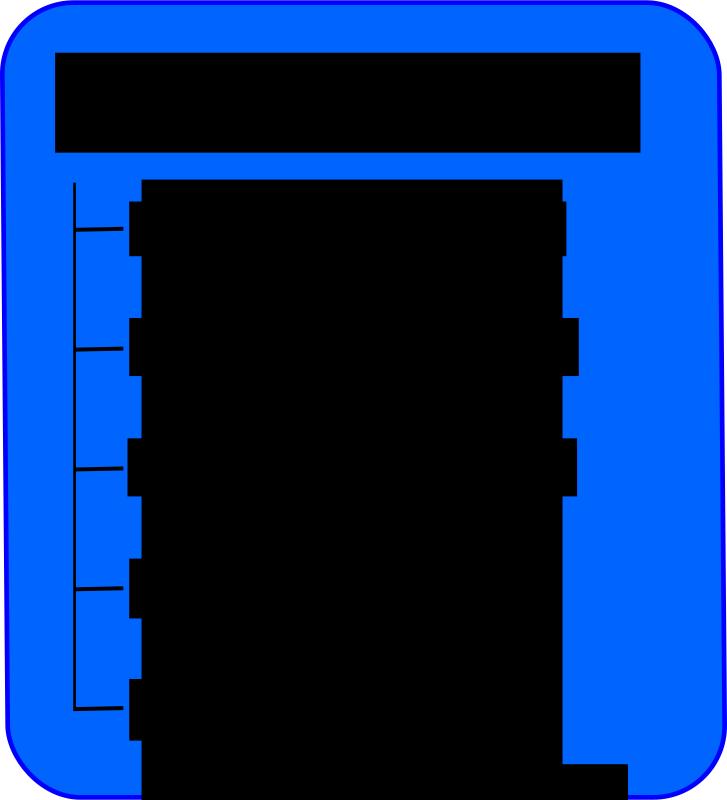
\includegraphics[width=\linewidth/2]{invariant.pdf} \caption{Important methods in Invariant 
class}\label{fig_invariant}
\end{center} 
\end{figure}
Invariants are only introduced after an initial solution to an instance is found and before the local 
search has begun. Invariants can represent either a variable or an auxiliary variable and are defined by oneway 
constraints. All Invariants must implement the methods \method{addChange}, \method{calculateDelta}, and 
\method{updateValue} that are used during local search. The \method{addChange} is used to tell an invariant that a 
variable in the oneway constraint defining it has been changed. The \method{calculateDelta} is used by the delta 
evaluation function in local search and updates the delta value of the invariant according to the changes 
received from \method{addChange}. The method \method{updateValue} is called when a move is performed to update the 
calue of the invariant. \\ 
Each type of invariant must implement its own method since the methods can be different for each type of invariant. \\ 
Some of the classes created in the \class{Local Search Engine} uses invariants but do not differentiate between them. 
If invariants did not have a common parent class then each invariant type would need its own data structure for 
storage. Another benefit is the search procedures do not have to exam which invariants the model consist of since they 
all have the same methods. It also makes it easier to add new invariants since all the functionality is implemented by 
the new invariant and nothing has to be changed in the Local Search Engine. \\ 
 

\label{sub_inv}
  \subsection{General Solver}
  The \gensol class contains the most high level methods and most of them are used directly by the user. An overview of 
the most important methods is shown in figure \ref{fig_general}. \\ \noindent
\begin{figure}[!b] 
\begin{center}
\includegraphics[width=0.8\linewidth]{general2.pdf} \caption{Important methods in General Solver class} 
\label{fig_general}
\end{center} 
\end{figure} 
The method \method{createVariables} takes three arguments to create a number of variables. The first argument 
is the number of variables to create with the given lower and upper bound, the second and third argument respectively. 
The method creates both the gecode variables used in the \class{Gecode Engine} and variables used in the \class{Local 
Search Engine} class. The variables used in the \class{Local Search Engine} class (LS variables) are of the class 
\class{Variable} and each has a pointer to the associated Gecode variable. The method returns pointers to the LS 
variables. \\ 
The method \method{relax} is only used if an initial solution could not be found within the limits given. It controls 
how the instance should be relaxed to find an initial solution. There is currently only one method implemented that 
relaxes the an instance that is described in subsection \ref{sub_inisol}. \\
All constraint available are created by calling the associated method in \gensol, that calls the constructor 
of the constraint and the method in \class{Gecode Engine} for posting the constraint in a Gecode space. The constraint 
objects should not be created directly by the user since these do not post the related constraint in the Gecode space. 
\\ 
To implements a new constraint object it must inheriting from the \class{Constraint} class 
and two methods, one in \class{General Solver} and one in \class{Gecode Engine}, must be implemented. The method in 
\class{Gecode Engine} must post the constraint in the \class{Gecode Engine} space. The method in \class{General Solver} 
should call the constructor of the constraint implemented and call the method in \class{Gecode Engine}. The solver must 
be able to reproduce the call to \class{Gecode Engine} in case it an initial solution is not found within the limits 
given. The relaxation method must be updated to handle the new constraint implemented as well. \boste{Could avoid 
inserting code in methods if constraints have pointers to the Gecode space but conceptually it does not make sense.} \\
To find an initial solution the method \method{initialSolution} must be called and it takes an integer argument. The 
argument indicates the time Gecode is allowed to search for an initial solution before \method{relax} is called. Once 
\method{relax} is called the same time limit is given again. \\
To find a better solution than the initial solution the method \method{optimizeSolution} can be called with a time 
limit as argument. That method starts the local search that is described in section \ref{sec_local}. \label{sub_gen}
  
\newpage
\section{Preprocessing and Initial Solution} \label{sec_gecode}
  All constraints that are created are both saved in \class{Storage} and parsed to \class{GecodeSolver}, that is derived 
from Gecode Space. In \class{GecodeSolver} they are posted such that Gecode can be used to find an initial solution. 
Gecode has a large selection of constraints that can be used \cite[p. 58-80]{MPG:M}. Most of the constructors of these 
constraints are overloaded such that they can take different arguments and works with different types of variables. 
  \subsection{Domain Reduction}
  When an initial solution to the model is requested, Gecode {\sffamily{Branch}} method is called that specifies which 
variables to branch on and what values should be examined in the branches. Gecode uses preprocessing before searching 
for a solution and that might reduce the domain of some of the variables. If the domain of a variable is reduced to a 
single value, the variable is said to be fixed and is assigned that value.   
  \subsection{Finding an Initial Solution}
  Once domain reduction preprocessing has been done a Gecode DFS search engine is started. The stop criteria for Gecodes 
search can be specified by an option class. A Gecode search engine takes a space and search option 
as arguments and the search option contains a stop object. The stop object can either be timestop, nodestop or 
failstop. Each time Gecode branches on a variable two new nodes are created and nodestop set a upper bound on the 
number of nodes to explorer. If Gecode reaches a node that gives an infeasible assignment to a variable then that space 
is failed and failstop sets an upper bound on the number of failed spaces that can occur before stopping. Timestop 
stops the search if the time limit is reach. \\ 
Instead of having only one of these stop object a multistop object has been created that combines all three stop 
objects if the user wants to having multiple stop criteria. \\ 
Combinatorial problems can be formulated with Gecode and these problems can be very difficult to solve. In these cases 
Gecode keeps searching for a solution until it finds one (or runs out of available memory). Instead, the search can be 
stopped using stop object and the constraints can be relaxed such that Gecode can find a initial solution to the 
instance. If one of the stop criteria is reached the \method{relax} is called and some of the constraint are relaxed. To 
relax some constraints a new Gecode Engine is created and all variables and constraints, except those relaxed, 
are created and added to the new space. In order to choose which constraint that should be removed the priority of the 
constraints, given by the user, is used. Different techniques can be applied for choosing which constraints with the 
same priority to remove. The one chosen here is a stepwise backward algorithm, that is a greedy approach. \boste{Article 
Marco talked about propose some method, but says a greedy approach is good as well? }. The number of constraints that 
are relaxed/removed is based on the number of constraints $|C|$ and the number of restarts made $r$. The number of 
relaxed constraints is given by equation (\ref{eq_relaxed}). 
\begin{equation}
 Relaxed = \ceil[\bigg]{\frac{2^{r}}{100}\cdot |C|}
 \label{eq_relaxed}
\end{equation} 
After six relaxations 64 \% of the constraints have been relaxed and if no solution can be found within the search 
limits, the search is stopped and finding a solution to the instance has failed.  \\ 
The constraints are chosen by their priority and ties are broken at random. I.e. a model with 100 constraint of 
priority 1, 40 of priority 2, and 15 of priority 3 and there are 20 constraints that should be relaxed. The 15 
constraints with priority 3 and 5 of the 40 constraints with priority 2 are chosen at random would not be posted. The 
constraints that are not posted in the Gecode space are still applied when doing local search, hence the initial 
solution might start with some violations.   \label{sub_inisol}

\newpage
\section{Structuring Local Search Model} \label{sec_ls}
Once an initial solution to the problem has been found by Gecode the model is transformed to create a model better 
suited for local search. \boste{talk briefly about DDG and propagation queue (what are they used for)} procedure can 
be split in several steps before the local search can begin. 
\begin{itemize}
  \item Define variables by one-way constraints
 \item Create invariants for the remaining constraints
 \item Create a dependency directed graph for variables and invariants
 \item Create propagation queue for all non fixed variables
%\item Initialize the invariants
% \item Initialize the constraints
% \item Initialize the objective function
\end{itemize}

  \subsection{Simplification}
  For each functional constraint $c_j$ two algorithm steps are used to create invariants, one checks if the constraint 
$c_j$ can be transformed into a oneway constraint and the other transforms $c_j$ into a one-way constraint defining 
$x_i$.  \\

\IncMargin{1em}
\begin{algorithm}[H]

%\SetKwFunction{relation}{relation}\SetKwFunction{coeff}{coefficient}
\SetKwFunction{makeOneway}{makeOneway}
\SetKwFunction{defi}{defines}
\algdata
\Input{\funccon $c_j$}
%\Output{Boolean}
\BlankLine
%\If{c \upshape already defines a oneway constraint}{\Return{} \false\; \boste{This constraint could be removed in 
%$O(\alpha(c_j))$}}
% \If{\upshape Number of integer variables not defined $> 1$}{\Return{} \false\; \boste{Needed in order to create the 
% right update queue}}
%\If{$|Y(c)| > 1$}{\Return{} \false}
%\If{\relation{c} \upshape is (==) }{\Return{} \true}
%\If{$c_j$ \upshape is not a linear equality}{
%  \Return{} \false}
%\int coeff = \coeff{c,v}\;
%\upshape in $\bigcup\limits_{o \in O} f_o(\vec{v})$}{	
%\tcp{Find the best variable to define}
\var $bestVariable$ = NULL\;
numberOfTies = 0 \;
\ForEach{$x_i$ \upshape in $X(c_j)$ }{
  \If{$x_i$ \upshape is fixed or defined}{
    \continue
  }
  \tcp{Break ties}
 % bestVariable = \decideBest{$x_i$,bestVariable} \;
  \If{\defi{$x_i$} $<$ \defi{$bestVariable$}}{
  \tcp{Choose the variable that helps define fewest invariants}
    $bestVariable$ = $x_i$ \;
    numberOfTies = 0 \;
%    \continue
  }
  \ElseIf{\defi{$x_i$} $==$ \defi{$bestVariable$}}{  
    \If{$|D(x_i)|$ $>$ $|D(bestVariable)|$}{
      \tcp{Choose the variable with largest domain size}
      $bestVariable$ = $x_i$ \;
      numberOfTies = 0 \;
 %     \continue
    } 
    \ElseIf{$|D(x_i)|$ $==$ $|D(bestVariable)|$}{  
      \If{$|deg(x_i)|$ $<$ $|deg(bestVariable)|$}{
	\tcp{Choose the variable with lowest degree} \boste{remember to define degree}
	$bestVariable$ = $x_i$ \;
	numberOfTies = 0 \;
%	\continue
      } 
      \ElseIf{$|deg(x_i)|$ $==$ $|deg(bestVariable)|$}{
	\tcp{Fair random} %\boste{Should this be further explained? (after alg)} 
	numberOfTies++ \;
	\If{Random(0,numberOfTies) == 0}{
	  $bestVariable$ = $x_i$ \;
	}
      }
    }
  }
}

\If{ bestVariable $\neq $ \upshape NULL}{
  \makeOneway{\Con $c_j$, \Var bestVariable} \;
 % \Return{} \true
}

%\Return{} \false \;
%\Return{} \true\;

\caption{canBeMadeOneway(\textsf{Constraint} $c_j$)} \label{algo_checkoneway} 
% \caption{Test if a constraint $c$ can define a variable $x$ } \label{algo_checkoneway}
\end{algorithm} \noindent
\DecMargin{1em} \\
For each functional constraint a non-fixed and non-defined variable is found if possible. If there is more than one 
eligible variable the best variable among those is found. The first tiebreaker is the number of oneway constraints the 
variable participate in (helps define other variables). The next tiebreaker is on the domain of the variables, the 
third is the number of constraints the variables participate in. If none of the tiebreakers can be used a fair random 
is used such that the probability is equal for all variables whose ties could not be broken. \\ 
Once a the best variable is found, if any, the algorithm \ref{algo_makeoneway}  \makeOneway is called.
%\begin{itemize}
% \item Highest search priority or highest domain size
% \item Lowest size of $C(x_i)$
% \item Fair random 
%\end{itemize}







%The variables that a constraint $c$ applies to is the scope $V(c)$. The constraints are of the type \class{Linear} and 
%a constraint $c$ have a right hand side $B(c)$. \\ 
\IncMargin{1em}
\begin{algorithm}[H]
\algdata
\Input{\Con $c_j$ and \Var $x_i$}
\Output{Updated $G$}
\BlankLine
set $Q$ \tcp*[r]{new coefficient set}
set $U$ \tcp*[r]{new variable set}
\tcp{Move $x_i$ to right hand side and set coefficient to 1}
\ForEach{$x_k$ \upshape in $X(c_j)\setminus {x_i}$}{
  $c'_{kj} = -\frac{c_{kj}}{c_{ij}}$ \;   
  $Q = Q\cup c'_{kj}$ \;
  $U = Q\cup x_k$ \;
}
\tcp{Move right hand side to left hand side and update coefficient}
double $b' = \frac{b(c_j)}{c_{ij}}$ \; \boste{Remember to define $b(c_j)$ before this}
\boste{coefficients can now be doubles (non integer)} \;
\textbf{invariant} $inv = $ new \Sum($U$,$Q$,$b'$)\; \tcp{Invariant that has the value (the sum of) the left hand 
side}
%$G$ = $G \cup \{inv\}$\; 
%$G$ = $G \setminus \{c_j\}$\; 
%$G$ = $G \setminus \{x_i\}$\;
  %\boste{Maybe remove $c$ from $G$}
  %\Return{\Sum{$V(c)$,$A(c)$,b}}

%\int $coef = A_{c,x}$\;
%$Q = A_c \backslash \{A_{c,x}\}$\;
%$U = V(c) \backslash \{x\}$\;
%\ForEach{$A_{c,x}$ \upshape in $Q$}{
%  $Q_{c,x} = A(c,x) \cdot \frac{-1}{coef}$
%}
%\int $b = B(c)$ \;
%\If{relation{c} \upshape is (==) }{
%  Invariant $c' = $ \Sum{$U$,$Q$,b}\;
%  $G$ = $G \cup c'$\; 
%  \boste{Maybe remove $c$ from $G$}
%  %\Return{\Sum{$V(c)$,$A(c)$,b}}
%}
%\Else{
%  Invariant $c' = $ \Sum{$U$,$Q$,b}\;
%  Invariant $c'' = $ \Max{c',lb(x)}\;
%  $G$ = $G \cup c'$\; 
%  $G$ = $G \cup c''$\; 
%  \boste{Maybe remove $c$ from $G$}
%  %\Return{\Max{inv,b}}
%}
 \caption{makeOneway(\textsf{Constraint} $c_j$, \textsf{Variable} $x_i$)} \label{algo_makeoneway}
\end{algorithm}\DecMargin{1em} \noindent
The algorithm transforms the constraint $c_j$ into a oneway constraint defining an invariant. The dependency directed 
graph $G$ is updated by adding the new invariant $inv$ and removing the constraint $c_j$ and variable $x_i$. \medskip 
\\ 
For each of the remaining constraints in $G$ auxiliary variables are introduced as invariants. In figure 
\ref{fig_smallG2} the invariant $i_2$ is an example of an auxiliary variable. The value of the invariant is the value 
of the left hand side of the corresponding constraint. These invariants are used to speed up local search, that is 
described in section \ref{sec_local}. \\


%\IncMargin{1em}
%\begin{algorithm}[H]
%\SetKwData{Oneway}{oneway}
%\SetKwFunction{makeOneway}{makeOneway}
%\SetKwFunction{Next}{next}\SetKwFunction{Constraints}{Constraints}\SetKwFunction{Remove}{remove}
%\SetKwFunction{canBeMadeOneway}{canBeMadeOneway}
%\algdata 
%\Input{A set $C$ of functional constraints sorted by increasing arity}
%\Output{A model better suited for local search}
%\BlankLine
%%\emph{special treatment of the first line}\;
%\Bool $change = $ \true\;
%\While{$C \neq \emptyset$ \textbf{and} $change$}{
%  $change = $\false \;
%  %\ForEach{$x \in X$}{
%  %  \upshape select \Var $x$ \upshape from $X$\;
%    \ForEach{\Con $c$ \upshape in $C$}{
%      \Bool $flag = $ \canBeMadeOneway{c}\;  
%      \If{$flag$}{
%	\makeOneway{c,x}\;
%	Remove $x$ from $X$\;
%	$change = \true$\;
%	\bre\;
%      }
%    }
%  }
%}
%\caption{Defining integer variables by one-way constraints}\label{makefunc}
%\end{algorithm}\DecMargin{1em}
%\noindent
%The following Two algorithms checks if the \cons $c$ can be transformed into a oneway constraint 
%and transforms $c_j$ into a one-way constraint defining $x$. 



%The algorithm creates invariants that defines variables $x_i \in X$ by one-way constraints. It uses two other 
%algorithms \canBeMadeOneway{$c_j$} and \makeOneway{$c_j$,$x_i$}. The first algorithm \\ 
%The complexity of algorithm \ref{algo_defintvar} depends on the complexity of the two other algorithms but for 
%simplicity let us assume they do not contribute for now. \\ 
%Let $\alpha_{max}$ be the largest arity among all constraints in $C$ and $n$ be the number of decision variables in 
%the 
%input set. The size of $X$ has decrease by at least one each time we pass line 3 except for the first time. Hence line 
%3 
%is passed at most $n$ times. Then the complexity of algorithm \ref{algo_defintvar} is $O(\alpha_{max} n^2)$. \\ 
%\medskip
%The coefficient of a variable $x_i$ in constraint $c_j$ is denoted $a_{ij}$. Let $\mathcal{F} = \{f_1,f_2,\dots 
%,f_k\}$ 
%be the family of objective functions \boste{Think we should discuss this Tuesday} and the coefficient of variable 
%$x_j$ in $f_k$ be $a_{kj}$. \boste{Maybe call it 
%evaluation functions. Does not make sense since $a_{34}$ refers both to constraint and obj. func} \\  



  \subsection{Dependency Digraph}
    \boste{What is the DDG? } \\ 
\boste{Why do we want a DDG?} \\
\boste{What properties should it have and why?} \\
The vertices $V$ in the dependency directed graph (\emph{DDG}) $G=(V,A)$ initially only represent the non-fixed 
variables and the constraints. The vertex $v \in V$ has an outgoing arc to vertex $u \in V$ if and only if the value of 
$u$ is directly dependent on the value of $v$. The variable vertices only have outgoing arcs and the constraints can 
only have ingoing arcs. The initial model will be modified by introducing invariants defined by oneway constraints and 
vertices representing invariants will be added to the graph $G$. \\
The graph can be illustrated with all the variable vertices to the left, all constraint vertices to the right and the 
invariants vertices are added between variables and constraint vertices.  \\  
The invariants are variables that are defined by oneway constraints or they can be auxiliary variables used in the local 
search. If a variable is defined by a oneway constraint the variable vertex is removed from $G$ since the value of that 
variable is no longer changed directly. \boste{is it clear what that means? (directly)} \\  
%From now on when talking about vertices in $G$ it refers to the variable, invariant or constraint it represents unless 
%other stated. \\
%The variables are non-fixed and non-defined and only have outgoing arcs. 
%Variables and invariants has an outgoing arc to the invariants that 
%depends on their value. \\ 
The DDG is used to update values of variables and invariants during local search. The graph $G$ is used to build the 
propagation queues described in subsection \ref{sec_propaqueue}. \\
The algorithms that creates invariants are described after this example. The example is a model with three variables 
and a two constraint and will illustrate how a possible dependency directed graph $G$ is made. 
\begin{center}
\begin{tabular}{rlr}
$ c_1: $&$2x_1 + x_2 - x_3 $&$= 2$ \\
$ c_2: $&$x_2 + x_3 $&$\leq 1$ \\
\end{tabular} 
\end{center}
Initially $G$ would consist of the three variables $x_1$, $x_2$, and $x_3$ and the constraints $c_1$ and $c_2$. The 
variable $x_3$ can be defined as an invariant $i_1$ by transforming $c_1$ to a oneway constraint. Once 
variable $x_3$ is defined by a oneway constraint it$c_1$ and $x_3$ are removed from the graph and replaced by invariant 
$i_1$. The variables $x_1$ and $x_2$ defines $i_1$ hence they have outgoing arcs to $i_1$. Invariant $i_1$ has an 
outgoing arc to $c_2$ since Variable $x_3$ participates in $c_2$.
\begin{center}
    \begin{tikzpicture}[scale=1]
        \vertex[label=$x_1$](x1) at (0,2) {};
        \vertex[label=$x_2$](x2) at (0,0) {};
        \vertex[label=$i_1$](i1) at (2,1) {};
        \vertex[label=$c_2$](c2) at (4,0) {};

    \tikzset{EdgeStyle/.style={->}}
        \Edge(x1)(i1)
        \Edge(x2)(i1)
        \Edge(x2)(c2)
        \Edge(i1)(c2)
        %\Edge(y1)(c3)
        %\Edge(y2)(c3)
    \end{tikzpicture}
        \captionof{figure}{Small example of DDG}
    \label{fig_smallG}
\end{center}
Auxiliary variable can be useful to speed up local search and in this example we could create an auxiliary 
variable $a_1$ which value is the sum of the left hand side of $c_2$. The auxiliary variable $a_1$ will be introduced 
by an invariant $i_2$ which will be added to $G$. The invariant $i_1$, representing $x_3$, and variable $x_2$ have 
an outgoing arc to $i_2$ and $i_2$ have an outgoing arc to $c_2$.
\begin{center}
%\begin{figure}[H]
    \begin{tikzpicture}[scale=1]
        \vertex[label=$x_1$](x1) at (0,2) {};
        \vertex[label=$x_2$](x2) at (0,0) {};
        \vertex[label=$i_1$](i1) at (2,1) {};
        \vertex[label=$i_2$](i2) at (4,0) {};
        \vertex[label=$c_2$](c2) at (6,0) {};

    \tikzset{EdgeStyle/.style={->}}
        \Edge(x1)(i1)
        \Edge(x2)(i1)
        \Edge(x2)(i2)
        \Edge(i1)(i2)
        \Edge(i2)(c2)
    \end{tikzpicture} 
    \captionof{figure}{Small example of DDG continued}
    \label{fig_smallG2}
 %   \end{figure}   \label{fig_smallG} 
\end{center}
When changing the value of $x_2$ both invariants need to be updated since they are dependent on the value of $x_2$. 
Invariant $i_2$ is dependent on the value of $i_1$ therefore to avoid updating $i_2$ twice, it is beneficial to update 
$i_1$ before updating $i_2$. This is the ordering the propagation queue gives which is discussed in the next 
subsection. \medskip \\ 
%\end{minipage}
%\boste{start on algorithms}
%The DDG $G$ is initially a bipartite graph where all the decision variables $X$ are vertices in one set and all the 
%constraints $C$ are vertices in the other set. If constraint $c$ applies to a variable $x$ then there is an arc from 
%the vertex representing $x$ to the vertex representing $c$. \\    
For each functional constraints $c_j$ two algorithms are used to create invariants, one checks if the constraint $c_j$ 
can be transformed into a oneway constraint and the other transforms $c_j$ into a one-way constraint defining $x_i$.  \\
%\IncMargin{1em}
%\begin{algorithm}[H]
%\SetKwData{Oneway}{oneway}
%\SetKwFunction{makeOneway}{makeOneway}
%\SetKwFunction{Next}{next}\SetKwFunction{Constraints}{Constraints}\SetKwFunction{Remove}{remove}
%\SetKwFunction{canBeMadeOneway}{canBeMadeOneway}
%\algdata 
%\Input{A set $C$ of functional constraints sorted by increasing arity}
%\Output{A model better suited for local search}
%\BlankLine
%%\emph{special treatment of the first line}\;
%\Bool $change = $ \true\;
%\While{$C \neq \emptyset$ \textbf{and} $change$}{
%  $change = $\false \;
%  %\ForEach{$x \in X$}{
%  %  \upshape select \Var $x$ \upshape from $X$\;
%    \ForEach{\Con $c$ \upshape in $C$}{
%      \Bool $flag = $ \canBeMadeOneway{c}\;  
%      \If{$flag$}{
%	\makeOneway{c,x}\;
%	Remove $x$ from $X$\;
%	$change = \true$\;
%	\bre\;
%      }
%    }
%  }
%}
%\caption{Defining integer variables by one-way constraints}\label{makefunc}
%\end{algorithm}\DecMargin{1em}
%\noindent
%The following Two algorithms checks if the \cons $c$ can be transformed into a oneway constraint 
%and transforms $c_j$ into a one-way constraint defining $x$. 



%The algorithm creates invariants that defines variables $x_i \in X$ by one-way constraints. It uses two other 
%algorithms \canBeMadeOneway{$c_j$} and \makeOneway{$c_j$,$x_i$}. The first algorithm \\ 
%The complexity of algorithm \ref{algo_defintvar} depends on the complexity of the two other algorithms but for 
%simplicity let us assume they do not contribute for now. \\ 
%Let $\alpha_{max}$ be the largest arity among all constraints in $C$ and $n$ be the number of decision variables in 
%the 
%input set. The size of $X$ has decrease by at least one each time we pass line 3 except for the first time. Hence line 
%3 
%is passed at most $n$ times. Then the complexity of algorithm \ref{algo_defintvar} is $O(\alpha_{max} n^2)$. \\ 
%\medskip
%The coefficient of a variable $x_i$ in constraint $c_j$ is denoted $a_{ij}$. Let $\mathcal{F} = \{f_1,f_2,\dots 
%,f_k\}$ 
%be the family of objective functions \boste{Think we should discuss this Tuesday} and the coefficient of variable 
%$x_j$ in $f_k$ be $a_{kj}$. \boste{Maybe call it 
%evaluation functions. Does not make sense since $a_{34}$ refers both to constraint and obj. func} \\  

\IncMargin{1em}
\begin{algorithm}[H]

%\SetKwFunction{relation}{relation}\SetKwFunction{coeff}{coefficient}
\SetKwFunction{makeOneway}{makeOneway}
\SetKwFunction{defi}{defines}
\algdata
\Input{\funccon $c_j$}
\Output{Boolean}
\BlankLine
%\If{c \upshape already defines a oneway constraint}{\Return{} \false\; \boste{This constraint could be removed in 
%$O(\alpha(c_j))$}}
% \If{\upshape Number of integer variables not defined $> 1$}{\Return{} \false\; \boste{Needed in order to create the 
% right update queue}}
%\If{$|Y(c)| > 1$}{\Return{} \false}
%\If{\relation{c} \upshape is (==) }{\Return{} \true}
%\If{$c_j$ \upshape is not a linear equality}{
%  \Return{} \false}
%\int coeff = \coeff{c,v}\;
%\upshape in $\bigcup\limits_{o \in O} f_o(\vec{v})$}{	

\tcp{Find the best variable to define}
\var bestVariable \;
numberOfTies = 0 \;
\ForEach{$x_i$ \upshape in $X(c_j)$ }{
  \If{$x_i$ \upshape is fixed or defined}{
    \continue
  }
  \tcp{Break ties}
 % bestVariable = \decideBest{$x_i$,bestVariable} \;
  \uIf{\defi{$x_i$} $<$ \defi{$bestVariable$}}{
  \tcp{Choose the variable that helps define fewest invariants}
    bestVariable = $x_i$ \;
    numberOfTies = 0 \;
    \continue
  }
  \uElseIf{\defi{$x_i$} $>$ \defi{$bestVariable$}}{
    \continue
  }
  
  \uIf{$D(x_i)$ $>$ $D(bestVariable)$}{
    bestVariable = $x_i$ \;
    numberOfTies = 0 \;
    \continue
  } 
  \uElseIf{$D(x_i)$ $<$ $D(bestVariable)$}{
    \continue
  }
  
  \uIf{$|C(x_i)|$ $<$ $|C(bestVariable)|$}{
    bestVariable = $x_i$ \;
    numberOfTies = 0 \;
    \continue
  } 
  \uElseIf{$|C(x_i)|$ $>$ $|C(bestVariable)|$}{
    \continue
  }
  \tcp{Fair random}
  numberOfTies++ \;
  \If{Random(0,numberOfTies) == 0}{
    bestVariable = $x_i$ \;
  }
}
\If{bestVariable \upshape found}{
  \makeOneway{\Con $c_j$, \Var bestVariable} \;
  \Return{} \true
}

\Return{} \false \;
%\Return{} \true\;

\caption{canBeMadeOneway(\textsf{Constraint} $c_j$)} \label{algo_checkoneway} 
% \caption{Test if a constraint $c$ can define a variable $x$ } \label{algo_checkoneway}
\end{algorithm} \noindent
\DecMargin{1em}
For each functional constraint a non-fixed and non-defined variable is found if possible. If there is more than one 
eligible variable the best variable among those is found. The first tiebreaker is the number of oneway constraints the 
variable participate in (helps define other variables). The next tiebreaker is on the domain of the variables, the 
third is the number of constraints the variables participate in. If none of the tiebreakers can be used a fair random 
is used such that the probability is equal for all variables which ties could not be broken. \\ 
Once a the best variable is found, if any, the algorithm \ref{algo_makeoneway}  \makeOneway is called.
%\begin{itemize}
% \item Highest search priority or highest domain size
% \item Lowest size of $C(x_i)$
% \item Fair random 
%\end{itemize}







%The variables that a constraint $c$ applies to is the scope $V(c)$. The constraints are of the type \class{Linear} and 
%a constraint $c$ have a right hand side $B(c)$. \\ 
\IncMargin{1em}
\begin{algorithm}[H]
\algdata
\Input{\Con $c_j$ and \Var $x_i$}
\Output{Updated $G$}
\BlankLine
set $Q$ \tcp*[r]{new coefficient set}
set $U$ \tcp*[r]{new variable set}
\tcp{Move $x_i$ to right hand side and set coefficient to 1}
\ForEach{$x_k$ \upshape in $X(c_j)\setminus {x_i}$}{
  $c'_{kj} = -\frac{c_{kj}}{c_{ij}}$ \;   
  $Q = Q\cup c'_{kj}$ \;
  $U = Q\cup x_k$ \;
}
\tcp{Move right hand side to left hand side and update coefficient}
double $b' = \frac{B(c_j)}{c_{ij}}$ \;
\boste{coefficients can now be doubles (non integer)} \;
\textbf{invariant} $inv = $ new \Sum($U$,$Q$,$b'$)\; \tcp{Invariant which value is (the sum of) the left hand side}
$G$ = $G \cup \{inv\}$\; 
$G$ = $G \setminus \{c_j\}$\; 
$G$ = $G \setminus \{x_i\}$\;
  %\boste{Maybe remove $c$ from $G$}
  %\Return{\Sum{$V(c)$,$A(c)$,b}}

%\int $coef = A_{c,x}$\;
%$Q = A_c \backslash \{A_{c,x}\}$\;
%$U = V(c) \backslash \{x\}$\;
%\ForEach{$A_{c,x}$ \upshape in $Q$}{
%  $Q_{c,x} = A(c,x) \cdot \frac{-1}{coef}$
%}
%\int $b = B(c)$ \;
%\If{relation{c} \upshape is (==) }{
%  Invariant $c' = $ \Sum{$U$,$Q$,b}\;
%  $G$ = $G \cup c'$\; 
%  \boste{Maybe remove $c$ from $G$}
%  %\Return{\Sum{$V(c)$,$A(c)$,b}}
%}
%\Else{
%  Invariant $c' = $ \Sum{$U$,$Q$,b}\;
%  Invariant $c'' = $ \Max{c',lb(x)}\;
%  $G$ = $G \cup c'$\; 
%  $G$ = $G \cup c''$\; 
%  \boste{Maybe remove $c$ from $G$}
%  %\Return{\Max{inv,b}}
%}
 \caption{makeOneway(\textsf{Constraint} $c_j$, \textsf{Variable} $x_i$)} \label{algo_makeoneway}
\end{algorithm}\DecMargin{1em} \noindent
The algorithm transforms the constraint $c_j$ into a oneway constraint defining an invariant. The dependency directed 
graph $G$ is updated by adding the new invariant $inv$ and removing the constraint $c_j$ and variable $x_i$. \medskip 
\\ 
For each of the remaining constraints in $G$ auxiliary variables are introduced as invariants. In figure 
\ref{fig_smallG2} the invariant $i_2$ is an example of an auxiliary variable. The value of the invariant is the value 
of the left hand side of the corresponding constraint. These invariants are used to speed up local search, that is 
described in section \ref{sec_local}. \\
In order to avoid circular definitions of invariants dependency directed graph $G$ should be acyclic. A circular 
definition could be if $x_i$ is used define $x_j$ and conversely \boste{vise versa?}. Then a change in value 
of $x_i$ would lead to a change in value of $x_j$ that again changes the value of $x_i$ and so on. \\ 
Once all invariants are introduced, $G$ is searched for strongly connected components of size two or more. A 
\emph{strongly connected component} (scc) is a maximal set of vertices $V^{SCC}$ such that for each pair of vertices 
$(u,v) \in V^{SCC}$ there exist both a path from $u$ to $v$ and a path from $v$ to $u$ \cite[p. 1170]{cormen}. 
To find all scc of size two or more Tarjan's algorithm \boste{cite SIAM J. Comput., 1(2), 146–160. Should I write the 
algorithm down as well?} that finds strongly connected components (\emph{scc}) is used. Each of these strongly 
connected components must be removed in order to keep $G$ acyclic, since a scc consist of at least one cycle. A scc can 
be removed \boste{made unstrongly connected?} by removing arcs and/or removing vertices. The arcs $A$ represents 
relations between variables, invariants and constraints and should not be changed. The vertices $V^{SCC}$ can only be 
vertices representing invariant since variable only have outgoing arcs and constraint only have ingoing arcs. In order 
to remove the strongly connected components one of the vertices could be removed that corresponds to undefine an 
invariant and reintroduce the transformed constraint and variable. Once these strongly connected components are removed 
there is still no guarantee that $G$ is a directed acyclic graph (DAG). A strongly connected component can be made of 
several cycles and there it might not be sufficient to remove a single vertex. using Tarjans algorithm and removal of 
strongly connected components is repeated until no strongly connected components of size two or more is found. \medskip 
\\ 
The first tiebreaker in algorithm \ref{algo_makeoneway} is used as a heuristic to reduce the number of cycles 
generated. If invariants are not used to define other invariants no cycles can occur, since cycles can only be made of 
invariant vertices. \\ 
Tarjans algorithm also gives each vertex representing invariants a time stamp that is used to create the propagation 
queues described in the next subsection. \\ 
\boste{Jeg føler det er meget rodet. Jeg ved ikke hvordan jeg skal dele det op}



%A circular definition could be if $x_i$ is used define $x_j$ and conversely \boste{vise versa?} then a change in value 
%of $x_i$ would lead to a change in value of $x_j$ that again changes the value of $x_i$ and so on. \\
%Cycles are found with . For each of the 
%strongly connected components of size two or more one of the vertices should be removed. Removing a vertex corresponds 
%to undefine an invariant and reintroduce the transformed constraint. After removing one vertex for each scc Tarjans 
%algorithm is used to find new scc if any. This is repeated until no scc of size two or more is found. Tarjans 
%algorithm 
%is modified a bit to give each vertex a time stamp when it becomes a part of a scc hence the last time it is visited. 
%This time stamp can be used for a topological sorting of the vertices once $G$ is a directed acyclic graph 
%(\emph{DAG}). 
%It gets complicated to compute the propagation queues if there exist a strongly connected component in $G$. 
%Only invariant vertices can be part of a strongly connected component of size at least two, since variables vertices 
%only have outgoing arcs and constraint vertices only have ingoing arcs. This indicates that there could be circular 
%definition of variables. Because of this we want to avoid ending up with strongly connected components in the graph 
%$G$. \medskip \\
%This is not the most efficient way of finding cycles, an algorithm with better complexity is described by \boste{cite 
%SIAM J. Comput., 4(1), 77–84, Tarjan has complexity O(|V|+|A|) not sure it is actually better to find elementary 
%cycles. Talk about finding minimum number of vertices to remove. Minimum feedback, NP-hard}. \\ 


%Consider the following three constraints as a small example. \boste{Should the example be introduced before the 
%algorithms?}
%\begin{center}
%\begin{tabular}{rlr}
%$ c_1: $&$2x_1 + y_2 -y_1 $&$= 2$ \\
%$ c_2: $&$2x_1 - y_2 $&$= 2 $ \\ 
%$ c_3: $&$x_1 +y_1 +y_2 $&$\leq 5 $
%\end{tabular} 
%\end{center}
%At first $y_1$ cannot be defined by a \oneway but $y_2$ can be defined by $c_2$ and then $y_1$ can be defined by 
%$c_1$. 
%The order in which the \oneway are created matters. \boste{Not finished here, continue tomorrow morning} 
%\begin{center}
%    \begin{tikzpicture}[scale=1]
%        \vertex[label=$x_1$](x1) at (-1,1) {};
%        \vertex[label=$y_1$](y1) at (3,2) {};
%        \vertex[label=$y_2$](y2) at (1,0) {};
%        %\vertex[label=$c_3$](c3) at (5,1) {};
%         %\vertex[label=$c_2$](c2) at (5,0) {};
%    \tikzset{EdgeStyle/.style={->}}
%        \Edge(x1)(y1)
%        \Edge(y2)(y1)
%        \Edge(x1)(y2)
%        %\Edge(x1)(c3)
%        %\Edge(y1)(c3)
%        %\Edge(y2)(c3)
%    \end{tikzpicture}
%\end{center}

%algorithm \ref{algo_defintvar} first check if $y_1$ can be defined by a \oneway which it cannot since $c_1$ applies to 
%two integer variables. Then $y_2$ cannot be defined by $c_1$ but can be defined by $c_2$. Then $c_2$ is transformed 
%into a \oneway $c_2'$ that defines $y_2$ and it is added to the DDG $G$, $c_2: y_2 = 2x_2 -2$. T  


% \floatname{algorithm}{Finding One-way constraints}
%\begin{algorithm}[ht]
% \caption{O$(|V|^2C_{mav}$O$($\method{canBeMadeOneway()}$)$}
% \begin{algorithmic}\label{updateGraph1}
%  \STATE{$Q = \emptyset$}
%  \STATE{$V = $ model.getVariables()}
%  \STATE{V.sort()}
%  \STATE{\bool change = \true }
%  \WHILE{change}
%    \FOR{\var var in $V$}
%      \FOR{\cons cons in var.usedInConstriant()}
%	\IF{\method{canBeMadeOneway(var, cons)}}
%	  \STATE{V.remove(var)}
%	  \STATE{$Q.psuhback($var$)$}
%	  \STATE{\Break }
%	\ELSE
%	\STATE{change = \\false}
%	\ENDIF
%      \ENDFOR
%    \ENDFOR
%   % \STATE{laxer$++$}
%%{$j\leftarrow 1$ \TO $i-1$}
%  \ENDWHILE
% \end{algorithmic}
%
%\end{algorithm}


% \floatname{algorithm}{}
%\begin{algorithm}[ht]
% \caption{\bool \method{canBeMadeOneway}(\var \text{var}, \cons cons) \qquad O$(V_{mav} + $O$($\method{makeOneway}$))$}
% \begin{algorithmic}\label{updateGraph1}
% \IF{cons.isOneway()}
%  \RETURN \\false
%  \ENDIF
% \STATE{\Int notDefined = 0} 
% \FOR { \var v in cons.getVariables}
% \IF{v.isInteger()}
%  \IF{!v.isDefinedBxOneway}
%  \STATE{notDefined++}
%  \ENDIF
%  \ENDIF
%  \IF{notDefined $> 1$}
%    \RETURN \\false  
% \ENDIF
% \ENDFOR
% \STATE{\Int coef = var.getCoefficient(cons)}
% \STATE{\Int objCoef = var.getObjectiveCoefficient()}
% 
% \IF{cons.Relation = EQ \OR coef$\cdot$objCoef $< 0$}
%    \STATE{\method{makeOneway}(\var var, \cons cons)}
%    \RETURN \true
% \ENDIF
% \RETURN \\false
% \end{algorithmic}
%\end{algorithm}


% \floatname{algorithm}{}
%\begin{algorithm}[ht]
% \caption{\method{makeOneway}(\var \text{var}, \cons cons) \qquad O$(V_{mav})$}
% \begin{algorithmic}\label{updateGraph1}
% \STATE{variables = cons.getVariables()-var}
% \STATE{coefficients = cons.getCoefficient-var.coefficients}
% \STATE{\Int coef = var.getCoefficient(cons)}
% \IF{coef $\neq$ -1}
% \STATE{coefficients = $\frac{-1}{coef}\cdot$ coefficients}
% \ENDIF
% \STATE{\invar invar$(variables, coefficients)$}
% \FOR{\var v in variables}
%  \IF{v.isDefinedBxOneway}
%    \STATE{\invar inv = v.oneway}
%    \STATE{inv.updateList.pushback(invar)}
%  \ELSE
%  \STATE{v.updateList.pushback(invar)}
%  \ENDIF
%   \ENDFOR
%   \STATE{cons.isOneway = \true }
%   \STATE{cons.defines = invar }
%   \STATE{var.setDefinedBx(invar,cons)}
%   \STATE{model.add(invar)}
%   \STATE{invar.currentvalue = -cons.getArgument(1)} 
% \end{algorithmic}
%\end{algorithm}
  

%First all integer variables $Y$ in the CSOP $\mathbb{P}$ \boste{Should I call the models CSOP or just model?} get 
%defined by oneway constraints by algorithm \ref{algo_makeints}. If some of the integer variables cannot be defined 
%\boste{Currently report fail and exit}. 
%\\ 
%\IncMargin{1em}
%\begin{algorithm}[H]
%\SetKwData{Oneway}{oneway}
%\SetKwFunction{makeIntVarOneway}{makeIntVarOneway}
%\SetKwFunction{Next}{next}\SetKwFunction{Constraints}{Constraints}\SetKwFunction{Remove}{remove}
%\SetKwFunction{intVarCanBeMadeOneway}{intVarCanBeMadeOneway}
%\algdata 
%\Input{A set $Y$ of integer variables sorted by decreasing domain size}
%\Output{A CBLS model for local search}
%\BlankLine

%\Bool $change = $ \true\;
%\While{$Y \neq \emptyset$ \textbf{and} $change$}{
%  $change = $\false \;
%  \ForEach{$y_i \in Y$}{
%    \upshape select \Var $y_i$ \upshape from $Y$\;
%    \ForEach{\Con $c_j$ \upshape in $C(y_i)$}{
%      \If{\intVarCanBeMadeOneway{$y_i$,$c_j$}}{
%	\makeIntVarOneway{$y_i$,$c_j$}\;
%	Remove $y_i$ from $Y$\;
%	isOneway($c_j$) = \true \;
%	$change = \true$\;
%	\bre\;
%      }
%    }
%  } \label{false}
%}
%\caption{Defining integer variables by one-way constraints}\label{algo_makeints}
%\end{algorithm}\DecMargin{1em}
%\noindent
%For each of the variables $y_i$ each of the constraints $c_j$ that applies to $y_i$ is checked if it can be made 
%oneway 
%to define $y_i$ until one is found or none can be found. This is done until there are no integer variables left or the 
%remaining integer variables cannot be defined, when the boolean change is false after line \ref{false}. Algorithm 
%\ref{algo_checkintoneway} checks if constraint $c_j$ can be made oneway to define $y_i$ and algorithm 
%\ref{algo_makeintoneway} transforms $c_j$ into a oneway constraint defining $y_i$ and updates the DDG $G$. \\
%Let $\mathcal{F} = \{f_1,f_2,\dots ,f_k\}$ be the family of objective functions. \\
%\IncMargin{1em}
%\begin{algorithm}[H]

%\SetKwFunction{relation}{relation}\SetKwFunction{coeff}{coefficient}
%\SetKwFunction{objcoeff}{objectiveCoefficients}
%\algdata
%\Input{\Var $y_i$ and \Con $c_j$}
%\Output{Boolean}
%\BlankLine
%\If{$c_j$ \upshape already defines a oneway constraint}{\Return{} \false\; \boste{This constraint could be removed in 
%$O(\alpha(c_j))$}}

%int $undefinedIntVar = 0$ \;
%\ForEach{\Var $x$ \upshape in $c_j$}{
%  \If{x is undefined integer variable}{
%    $undefinedIntVar++$\;
%  }
%}
%\If{$undefinedIntVar > 1$ \label{undefined}}{\Return{} \false  \boste{Insures no cycle is created} \; 
%\tcp {else only $y_i$ is undefined integer variable}} 
%\If{$c_j$ \upshape is linear equality}{\Return{} \true}
%\If{\upshape coefficient $c_{ij} \geq 0 $ \label{positivecoef}}{ 
%  \Return{} \false \; 
%}
%\ForEach{ $f_j$  in $\mathcal{F}$ }{
% \If{$f_ij < 0$ \label{objectivecoef}}{
%    \Return{} \false \;
%    \boste{Not sure of to define coefficients in objective functions. coefficient of variable i in constraint j could 
%be $c_{ij}$ but $c_j$ is used for constraint and then all variable $y_i$ should be $y_i$}
%  }
%}
%\Return{} \true\;
% \caption{intVarCanBeMadeOneway( \textsf{Variable} $y_i$, \textsf{Constraint} $c_j$)} \label{algo_checkintoneway}
% \caption{Test if a constraint $c$ can define a variable $x$ } \label{algo_checkoneway}
%\end{algorithm}
%\DecMargin{1em}
%If constraint $c_j$ already defines another variable it cannot be used to define $y_i$. Line \ref{undefined} makes 
%sure 
%that integer variable $y_i$ is not defining another integer variable $y_k$. This limits the model and increases the 
%complexity of algorithm \ref{algo_makeints} because of the addition of the initial while loop. The 
%condition in line \ref{undefined} makes sure that no strongly connected component of size 2 or greater is created in 
%$G$. \boste{This should be described why we dont want that and what a SCC is}. The lines \ref{positivecoef} and 
%\ref{objectivecoef} returns false if the coefficient of $y_i$ in $c_j$ is positive or one of the coefficients in the 
%objective functions is negative. If that is not the case the constraint $c_j$ can define variable $y_i$ since we 
%restrict the lower bound of $y_i$ by the oneway constraint and want to minimize its value in the objective functions. 
%This gives some other complications which will be described after algorithm \ref{algo_makeintoneway}. \\ 
%\IncMargin{1em}
%\begin{algorithm}[H]
%\algdata
%\Input{\Var $y_i$ and \Con $c_j$}
%\Output{Updated $G$}
%\BlankLine
%%\int $coef = A_{c,x}$\;
%set $Q$ \tcp*[r]{new coefficient set}
%set $U$ \tcp*[r]{new variable set}
%\tcp{Move $y_i$ to right hand side and set coefficient to 1}
%\ForEach{$x_k$ \upshape in $X(c_j)\setminus {y_i}$}{
%  $c'_{kj} = -\frac{c'_{kj}}{c_{ij}}$ \;   
%  $Q = Q\cup c'_{kj}$ \;
%  $U = Q\cup x_k$ \;
%}
%\tcp{Move right hand side to left hand side and update coefficient}
%double $b' = \frac{B(c_j)}{c_{ij}}$ \;
%\boste{coefficients can now be doubles (non integer)} \;
%\If{$c_j$ \upshape is linear equality}{
%  \textbf{invariant} $inv = $ new \Sum($U$,$Q$,$b'$)\;
%  $G$ = $G \cup \{inv\}$\; 
%  $G$ = $G \setminus \{c_j\}$\; 
%  %\boste{Maybe remove $c$ from $G$}
%  %\Return{\Sum{$V(c)$,$A(c)$,b}}
%} \Else {
%    \boste{Remember to say all constraints are either LQ or EQ} \;
%    \textbf{invariant} $ inv= $ new \Sum($U$,$Q$,$b'$)\;
%    \textbf{Invariant} $ inv' = $ new \Max{$inv$,lowerbound($y_i$)}\;
%    $G$ = $G \cup inv$\; 
%    $G$ = $G \cup inv'$\; 
%    $G$ = $G \setminus \{c_j\}$\; 
% \boste{Maybe remove $c$ from $G$}
  %\Return{\Max{inv,b}}
%}

% \caption{makeIntVarOneway(\textsf{Variable} $y_i$, \textsf{Constraint} $c_j$)} \label{algo_makeintoneway}
% %\caption{Make one-way constraint from $c$ defining variable $x$ } \label{algo_makeoneway}
% \end{algorithm}\DecMargin{1em} \noindent 
%If the constraint $c_j$ is a linear equality constraint, an invariant $inv$ is defined by a new oneway constraint. The 
%oneway constraint is made by isolating $y_i$ on the right side in $c_j$. Then $inv$ is added to $G$ and $c_j$ is 
%removed from $G$. \\ 
%If $c_j$ is not a linear equality constraint then it is a linear constraint with an upper bound $B(c_j)$. Since 
%$c_ij$, 
%the coefficient of $y_i$, in $c_j$ is negative $y_i$ can be isolated on the right hand side as an upper bound. The 
%coefficients of $y_i$ in the objective functions are non-negative, know from algorithm \ref{algo_checkintoneway} line 
%\ref{objectivecoef}. Variable    


 \label{sec_ddg}
  \subsection{Propagation Queue}  
    For each independent variable $x_i$ a propagation queue $q_i$ is made. A propagation queue $q_i$ is an 
topological sorting of invariants that are reachable from the vertex representing $x_i$ in the dependency directed 
graph $G$. The vertices in the propagation queue are ordered according to their time stamp in decreasing 
order which is a topological sorting such that there is no backward pointing arc. \\
The propagation queue $q_i$ is used such that each invariant dependent on the value of $x_i$ is updated at most once if 
the variable changes value. The DDG represents which invariant that are directly affected by a change in variable $x_i$ 
but not the order in which they should be updated. Figure \ref{fig_propqueue} shows the necessity of such an ordering. 
\\
\begin{figure}[b]
\centering
\begin{tikzpicture}[scale=1]
        \vertex[label=$x_1$](x1) at (0,2) {};
        \vertex[label=$y_2$](i2) at (2,1) {};
        \vertex[label=$y_1$](i1) at (4,2) {};
        %\vertex[label=$y_3$](i3) at (5,1) {};
         %\vertex[label=$c_2$](c2) at (5,0) {};
    \tikzset{EdgeStyle/.style={->}}
        \Edge(x1)(i1)
        \Edge(x1)(i2)
        \Edge(i2)(i1)
        %\Edge(x1)(c3)
        %\Edge(y1)(c3)
        %\Edge(y2)(c3)
\end{tikzpicture}  \caption{Importance of propagation queue} \label{fig_propqueue}
\end{figure} 
If $y_1$ is updated before $y_2$ then it might need to be updated again after $y_2$ is updated hence updated 
twice. In worst case the number of updates performed when updating $x_i$ could be exponential in the number of vertices 
reachable from $x_i$ instead of linear. \\ 
Once the dependency directed graph is a DAG each invariant vertex has been given a time stamp by Tarjans algorithm. 
Propagation queues are implemented as red-black trees without duplicates hence they have insert time complexity 
$O(log(n))$. For each variable vertex $v_i$ in dependency digraph $G$ a depth first search is made. Each vertex 
visited is added to the propagation queue of $v_i$. This gives a time complexity of $O(rlog(r))$ where $r$ is the 
number of reachable vertices from $v_i$.  \medskip \\ 
During local search when a single variable $x_i$ changes value the change propagate through the DDG using 
the ordering from the propagation queue $q_i$. When two or more variable change value the propagation queues can be 
merged into a single queue removing duplicates.  \\ 
Figure \ref{fig_ddgs} and \ref{fig_props} gives an example of creating a propagation queue for a variable based on the 
dependency graph. It is possible to create different propagation queues from the example but we do not differentiate 
between them as long as there is no backward going arc. In this case we have single variable $x_1$ that creates the 
propagation queue $q_1 = [y_2,y_1,y_4,y_3,y_5]$. The idea is to send the changes from $x_1 $ to $y_2$,$y_1$, and $y_4$ 
then go to $y_2$ update its value and send the change to $y_5$. Go to $y_1$, update and send change, go to $y_4$ etc.  
\begin{figure}[!t]
\centering
\includegraphics[width=\linewidth]{1.pdf} \caption{Example of subgraph in the DDG.}\label{fig_ddgs}
% \end{center} 
\end{figure}
\begin{figure}[!b]
\centering
\includegraphics[width=\linewidth]{2.pdf} \caption{Example of a propagation queue created from figure
\ref{fig_ddgs}.} \label{fig_props}
% \end{center} 
\end{figure}\label{sec_propaqueue}
    
  
\newpage  
\section{From Modeling to Local Search}
Simple problem will be modeled in this section and the different parts of this constraint based local search solver 
will be illustrated. \\
\boste{New subsection- The problem} \\ 
A city have budget of 50 million kr. for a festival and have some suggested activities. The activities have 
an individual cost and have been given a score based on how successful the activity is expected to be. The duration of 
the festival is three weeks and the activities have individual requirement to which week the can be planned. Exactly 
two must be planned the first week, at most two the second week and at most one the third week. The job is to 
plan activities with in the budget and schedule maximizing the score. Table \ref{tab_activity} shows the data given. \\
\begin{table}[b]
\centering
\begin{tabular}{|l|l|l|l|l|l|}
\hline
Activity No. & Cost & Score & Week 1 & Week 2 & Week 3 \\ \hline
1            & 20   & 3     & yes    & yes    & no     \\ \hline
2            & 10   & 2     & yes    & no     & no     \\ \hline
3            & 35   & 4     & no     & no     & yes    \\ \hline
4            & 42   & 5     & yes    & yes    & yes    \\ \hline
5            & 13   & 2     & no     & yes    & no     \\ \hline
6            & 37   & 4     & yes    & no     & yes    \\ \hline
\end{tabular}
\caption{Suggested activities}
\label{tab_activity}
\end{table} \noindent
If an activity is chosen it is chosen for all the weeks with yes. \\ 
\boste{Section - Model}
Each of the activities can be represented by a binary variable whether the activity is chosen or not. The constraint of 
each week can be modeled with the \class{Linear} constraint \boste{Somewhere I should describe the constraints and 
invariants implemented}. 
\newpage
\section{Local Search and Metaheuristics} \label{sec_local}
  The \class{LocalSearchEngine} class uses the model created for local search described in section \ref{sec_ls} and 
uses local search to improve the initial solution. The vector holding pointers to the independent variables is given a 
random ordering, called a mask, that is used in local search. \\
Local search explores how changing the value of few variables will affect the solution quality, hence exploring a 
neighbor 
solution. The key for being efficient is to compute this change fast. The dependency digraph and the propagation 
queues are used for this. Before committing a neighborhood operation several neighborhood operations might be explored 
before choosing one to commit. To evaluate a neighborhood operation a delta value for each invariant is used. The 
delta value is the value an invariant would change if the neighborhood operation is committed. By this we can evaluate 
the neighbor solution without committing a neighborhood operation. \\
Each constraint $c \in C$ created in the model was given a priority $p$ and these priorities are used during local 
search. Let $k$ denote the highest priority given. A new \class{Sum} invariant is created for each priority $p$ and 
one for the objective function. This is done at the same time invariants are created by each constraint class. \\
Let $q_p \in Q$ be the sum of violation degree of the constraints with priority $p$. The objective functions 
value is consider as $q_0$ and the vector $Q$ is used to evaluate the quality of a solution. The evaluation function 
$f(\tau)$ is not returning a single value but the quality vector, $f(\tau) = Q_\tau$.  \\ 
Two candidate solutions $\tau$ and $\tau'$ each have a vector of quality $Q_\tau$ and $Q_{\tau'}$ respectively. To 
determine which of the two solution are best their vector can be compared, starting with position $k$ and going 
backwards. The first time they differ in value determine which solution is best, the one with the lowest value. 
Illustrated with a small example:
\begin{align}
 Q_\tau &= (5,2,4,2) \\ 
 Q_{\tau'} &=(10,6,3,2) 
\end{align}
Violation degrees of constraints with priority 3 ($Q_\tau[3]$, $Q_{\tau'}[3]$) contributes with 2 in each candidate 
solution and then the violation degree of constraints with priority 2 is consider. Then candidate solution $\tau'$ is 
consider better than $\tau$ since $Q_\tau(2) = 4$ $>$ $Q_{\tau'}(2) = 3$. \\
The new classes used for local search are in three different categorize; moves, neighborhoods, and search 
procedures. A \class{Move} object stores information of a neighborhood operation including the change of the evaluate 
function. A subclass of the \class{Neighborhood} class is the choice of neighborhood function and gives the 
sequence in which the neighbor solutions in the neighborhood graph are explored. The search procedures can query a 
\class{Neighborhood} class to evaluate a neighborhood operations, a \class{Move} class, effect on the evaluation 
function. The search procedures determine which neighborhood operation to commit, if any. Neighborhoods and 
search 
procedures are combined to create different local search algorithms and \class{LocalSearchEngine} uses them within the 
time limit to search for a better solution. \\
The first algorithms that is used is a first improvement until a local optmia is found. Gecode is not used to optmize 
hence it might be posible to improve the initial solution very easily. If Gecode does not find an initial solution it 
is very likely that the construction heuristic, random assignment, does not give a feasible solution and is far from a 
local optima. It is prefered to start in local optima or at least close to one and first improvement is very efficient 
at finding a local optima. \\
\begin{figure}[!t]
\begin{center}
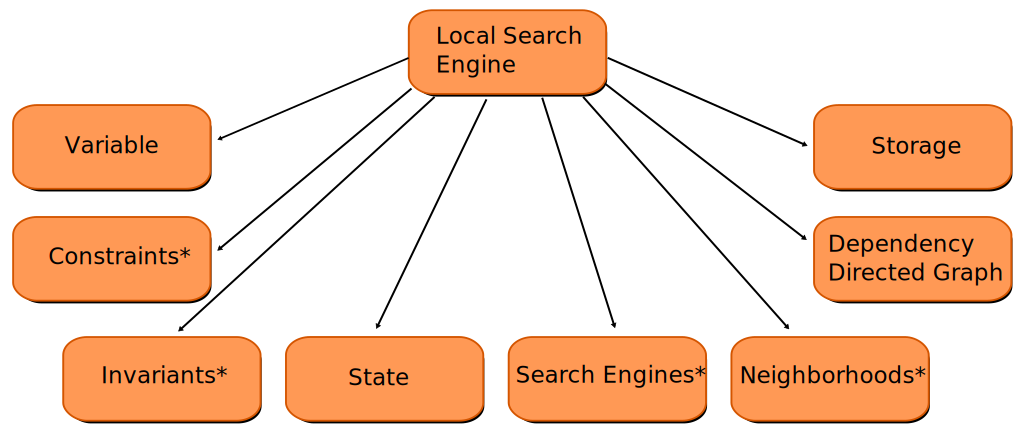
\includegraphics[width=0.9\linewidth]{LSE}\caption{Overview of the class pointers of \class{LocalSearchEngine}. The 
fields marked with a star (*) are several classes of that type.} 
\label{fig_lse}
\end{center}
\end{figure}\noindent




% For simplicity let us first consider the neighborhood operation involving changing the value 
% of a single 
% variable $x$. The change of variable value is send through the dependency digraph where each invariants, reachable from 
% the vertex representing $x$, is updated. The propagation queue is used to determine the sequence the invariants should 
% be updated. This will update invariants that represent violation of constraints with different priority and the 
% evaluation function. \\
% If a neighborhood operation consist of more variables changing values, such as swapping values of two variables, the 
% propagation queues 
% of these variables can be merged. The merging should remove duplicates and keep the invariants topological sorted. The 
% invariants unique time stamp can be used to keep the ordering. The new queue gives an ordering the invariants should be 
% updated such that they are only updated once during each neighborhood operation. \\ 
  \subsection{Neighborhoods}
  The neighborhood classes are all subclasses of the super class \class{Neighborhood} such that they can easily be 
combined with the search procedures. The methods of neighborhoods are illustrated in figure \ref{fig_neighborhood}. \\
\begin{figure}[!b]
\begin{center}
\includegraphics[width=0.9\linewidth]{neighborhood}\caption{The methods all Neighborhood classes needs to implement.} 
\label{fig_neighbborhood}
\end{center}
\end{figure}
All \class{Neighborhoods} implemented uses a step functions that changes value of a single independent variable, from 
0 to 1 or vise versa since all variables are binary. A neighborhood operation is stored in an a \class{Move} that 
contains a pointer to the variable used, the variables change in value, and the change to the quality vector $Q$, 
once computed. The change in the quality vector is referred to at the \emph{delta vector}. \\ 
The \class{Neighborhood} classes that are implemented are shown in table \ref{tab_neighb}. \\  
\begin{table}[!t]
\centering
\begin{tabular}{|l|l|}
\hline
class                          & Heuristic                                          \\ \hline
\class{FlipNeighborhood}     & All variables                                      \\ \hline
\class{RestrictedFlipNE}     & A Random subset of the variables	               \\ \hline
\class{ConflictOnlyNE}       & Variables in unsatisfied constraints           \\ \hline
\class{RandomConflictFlipNE} & Variables from a random unsatisfied constraint \\ \hline
\end{tabular}
\caption{Table of \class{Neighborhood} classes}
\label{tab_neighb}
\end{table}
The method \method{next()} creates new \class{Move} object and returns a pointer to it. If all the 
different neighborhood operation has been returned the method returns a pointer to \textbf{NULL} instead. To know when 
a neighborhood has been fully explored, counters and iterators are used depending on the neighborhood. These are 
reseted when returning \textbf{NULL} or the method \method{commitMove(move)} is called. The \class{Move} created only 
contain the variable and its suggested change in value, the delta vector is not computed yet. \\ 
Method \method{nextRandom()} gives a random neighborhood operation without changing the.  \\ 
Method \method{calculateDelta(move)} takes a \class{Move} pointer as argument and propagate the change through the 
dependency digraph using the propagation queue of the variable. The method identical for all the \class{Neighborhood} 
classes implemented. A neighborhood operation that calculate the delta change if variable $x_i$ would change value is 
describe with the following step:
\begin{enumerate} 
 \item Reset delta value of invariants in quality vector $Q$
 \item Send delta value of $x_i$ to neighbor invariant in DDG.
 \item For each invariant $inv$ in propagation queue of $x_i$, calculate $inv$s delta value, if it is not zero, send 
it to neighbor invariants in DDG. 
 \item If a variables delta value is not allowed, by a oneway constraint, reset all delta values of invariant in 
the propagation queue.
 \item Otherwise set $move$s delta quality vector. 
\item return if the $move$ is an allowed neighborhood operation. 
\end{enumerate}
The delta values of the invariants can be reset by calculating delta value, when no change is send. The reason for 
resetting them is only to make sure their queue of changes is empty before the next neighborhood operation. \\ 
To perform a step the method \method{commitMove(move)} is called with a pointer to the \class{Move} that used be used.  
\method{commitMove(move)} use the delta value calculated by \method{calculateDelta(move)} to update the value of 
invariants. The delta value needs to be recomputed since other neighborhood operation might have been suggested. Once 
the delta values of invariants have been computed they can be added to their current value. Invariants that represent 
violation of a single constraint are kept in a hash map of they are non zero. If they change value from non zero to zero 
or vise versa, that hash map needs to be updated. The hash map is used by the two neighborhoods \class{ConflictOnlyNE} 
and \class{RandomConflictFlipNE} that only can be used when the current solution is infeasible. \\
A default method \method{compareMoves(move1,move2)} compares the delta vector of two \class{Move} pointers and returns 
0 if they are the same, 1 if if move1 is best and 2 otherwise. \\ 
The size of the neighborhood and the restriction applied to it, if any. Method \method{getSize()} returns the size of 
the current neighborhood, for \class{ConflictOnlyNE} and \class{RandomConflictFlipNE} the neighborhood size can change 
after each step. \\ 





  \subsection{Search Procedures}
  \class{Neighborhood} classes do not implement any strategy of which neighborhood operation to choose. 
Search procedures are using a \class{Neighborhood} and define this strategy. The classes implemented 
are \class{FirstImprovement}, \class{BestImprovement}, \class{TabuSearch}, and \class{RandomWalk}. \\
\class{FirstImprovement}, \class{BestImprovement}, and \class{RandomWalk} are implementation of local search 
algorithms of almost same name and can be used together with any of the \class{Neighborhood} classes. 
\class{TabuSearch} is an implementation of the metaheuristic tabu search using a tabu tenure, and 
an aspiration criteria. \medskip \\
The class \class{BestImprovement} looks at each \class{Move} a \class{Neighborhood} class $NE$ gives and finds uses the 
\class{Move} that leads to the best solution. The best \class{Move} is determined from their delta vector after the 
method \method{calculateDelta()} of the \class{Neighborhood} is called on each \class{Move} returned by the 
neighborhood until \textbf{NULL} is returned. \class{BestImprovement} returns a flag that tells if the current 
solution was improved. A flag can be given to \class{BestImprovement} that indicate if it should commit a non 
improving \class{Move}. How each iteration is done is describe by algorithm \ref{algo_BI} \\ 
\IncMargin{1em}
\begin{algorithm}[H]

%\SetKwFunction{relation}{relation}\SetKwFunction{coeff}{coefficient}
\SetKwFunction{makeOneway}{makeOneway}
\SetKwFunction{defi}{defines}
\algdata
\Input{\bool alwaysCommit, \class{Neighborhood} NE}
\Output{\bool improvement}
\BlankLine
%\If{c \upshape already defines a oneway constraint}{\Return{} \false\; \boste{This constraint could be removed in 
%$O(\alpha(c_j))$}}
% \If{\upshape Number of integer variables not defined $> 1$}{\Return{} \false\; \boste{Needed in order to create the 
% right update queue}}
%\If{$|Y(c)| > 1$}{\Return{} \false}
%\If{\relation{c} \upshape is (==) }{\Return{} \true}
%\If{$c_j$ \upshape is not a linear equality}{
%  \Return{} \false}
%\int coeff = \coeff{c,v}\;
%\upshape in $\bigcup\limits_{o \in O} f_o(\vec{v})$}{	
%\tcp{Find the best variable to define}
\class{Move} bestMove = NE.next() \;
\class{Move} move = NE.next() \;
\While{move $\neq$ NULL}{
  \bool allowed = NE.calculateDelta(move) \;
  \If{!allowed}{
    move = NE.next() \;
    \continue \;
  }
  bestMove = compareMove(move,bestMove) \;  
  move = NE.next() \;
}
\bool improvement = Check if bestMove gives improvement \;
\tcp{by looking at delta vector} \;
\If{improvement \textbf{OR} alwaysCommit}{
  NE.commitMove(bestMove)
 }
\Return improvement \;

\caption{BestImprovement Start} \label{algo_BI} 
 %\caption{Test if a constraint $c$ can define a variable $x$ } \label{algo_checkoneway}
\end{algorithm} \noindent
\DecMargin{1em} \\
If \class{BestImprovement} is combined with the neighborhood class \class{RandomConflictConNE} it gives a minimim 
conflict heuristic that can be useful to reach a feasible solution. \\ 
\class{FirstImprovement} has an implementation very similar to \class{BestImprovement}. Instead of calculating each 
\class{Move} of a \class{Neighborhood} class $NE$ it stops requesting a \class{Move} once an improving \class{Move} is 
found. If no improving \class{Move} is found, when $NE$ returns a \textbf{NULL} pointer it does not commit a 
\class{Move}. If no improving \class{Move} is found the current solution is in a local optima with the regard to the 
chosen \class{Neighborhood} class. \\ 
The class \class{RandomWalk} uses the method \method{nextRandom()} from its \class{Neighborhood} $NE$ and if that 
\class{Move} is allowed it is committed. It takes an integer as argument that indicate the number of times it is 
repeated. The benefit is many iteration can be done but they are not as likely to have a good quality.  
Though tabu search is a metaheuristic it is implemented the same way as the other search procedures but with some 
additions. It takes four arguments; the number of iterations made so far, the best solution found, the current 
solution, and a tabu list. The implementation is similar to \class{BestImprovement} with additional checks with regard 
to the tabu list and aspiration criteria. The aspiration criteria is if a neighborhood operation is tabu but leads to a 
solution better than one found so far, the tabu list is ignored and that neighborhood operation is done. The 
tabu list has size $n$ and each variable has a integer corresponding to the last iteration that variable was 
changed. The tabu tenure is chosen to be based on the neighborhood size with a small degree of random. $tt = 
random(0,10) + min(2\cdot neigborhood size, n/200)$. The neighborhood size might be very small when only considering 
variables that are in a conflicting constraint, hence the multiplier. \\ 
The algorithm for tabu search for a single flip neighborhood sketched by algorithm \ref{algo_TS}. \\ 
\IncMargin{1em}
\begin{algorithm}[H]

%\SetKwFunction{relation}{relation}\SetKwFunction{coeff}{coefficient}
  \algdata
\Input{\int iteration, int[] best, int[] current, int[] tabulist }
%\Output{\bool improvement}
\BlankLine
\int tabuTenure = Random(0,10)+ min(NE.getSize()*2, tabulist.size() /200) \;
\class{Move} bestMove = NE.next() \;
\class{Move} move = NE.next() \;
\While{move != NULL}{
  \bool allowed = NE.calculateDelta(move) \;
  \If{!allowed}{
    move = NE.next() \;
    \continue \;
  }
  \bool isTabu = (iteration - tabulist[move.ID]) $<=$ tabutenure \;
  \If{isTabu}{
    \If{betterThanBest(current,move.getDeltaVector(), best)}{
      NE.commitMove(move)
      tabulist[move.ID] = iteration \;
      \Return \true \;
      
    }{
      move = NE.next() \;
      \continue \;
    }  
  }
  bestMove = compareMove(move,bestMove) \;  
  move = NE.next() \;
}
%\bool improvement = Check if bestMove gives improvement to current solution 
%\tcp{by looking at delta vector} \;
NE.commitMove(bestMove) \;
%\Return improvement \;

\caption{TabuSearch Start(iteration, best,current,tabulist)} \label{algo_TS} 
 %\caption{Test if a constraint $c$ can define a variable $x$ } \label{algo_checkoneway}
\end{algorithm} \noindent
\DecMargin{1em} \\
\class{TabuSearch} needs to be combined with a \class{Neighborhood} class that uses single flip neighborhood operation. 
This makes it less flexible in combining it with a \class{Neighborhood} class than the other search procedures 
\class{FirstImprovement}, \class{BestImprovement}, and \class{RandomWalk}. \\ 
In order to create an efficient local search we need to change search procedure at some point, with the exception of 
tabu search that can perform well on it own. 




  \subsection{Local Search Algorithms}
  When a model better suited for local search has been made, the remaining time is used to do local search. The 
algorithms check if the timelimit is reach before each iteration of a search procedure. The best solution found while 
searching is saved in a \class{State} class such that the search can continue but always report the best solution when 
the time limit is reached. \\ 
Three algorithms have been made from combining \class{Neighborhood} classes and search procedures that will be used to 
test efficiency of the framework. The first algorithm uses two \class{TabuSearch} with different 
\class{Neighborhood} classes. When the solution is infeasible \class{TabuSearch} is combined with \class{ConflictOnlyNE} 
to only look at variables that can reduce the number of violations. When the current solution is feasible 
\class{TabuSearch} with a \class{RestrictedFlipNE} class is used. If the number of independent variables are less than 
or equal to 5000 it uses a \class{FlipNeighborhood} class instead. The reason for choosing a subset of the neighborhood 
to examine is to increase the number of iterations made in case the neighborhood is large. \\
\IncMargin{1em}
\begin{algorithm}[H]

%\SetKwFunction{relation}{relation}\SetKwFunction{coeff}{coefficient}
  \algdata
%\Input{\int iteration, int[] best, int[] current, int[] tabulist }
%\Output{\bool improvement}
%\BlankLine
\class{ConflictOnlyNE} CON \;
\class{RestrictedFlipNE} RFN \;
\class{TabuSearch} TSCON(NE) \;
\class{TabuSearch} TSRFN(NE2) \;
\int iteration = 0 \;
\int[] best = getSolution() \;
\int[] current = getSolution() \;
\int[] tabulist(neighborhood.getSize(), -neighborhood.getSize()) \;
\While{\upshape within time limit}{
  \eIf{\upshape Current solution is feasible}{
    TSCON.start(iteration ,current, best, tabulist) \;
    iterations++ \;     
    \If{\upshape getSolution() is better than bestSolution} {
      bestSolution = getSolution() \;
    }
  }{
    TSRFN.start(iteration, current, best, tabulist) \;
    iterations++ \;     
    \If{\upshape getSolution() is better than bestSolution} {
      bestSolution = getSolution() \;
    }
  }
}
\caption{Local Search - Test Algorithm 1} \label{algo_LS1} 
 %\caption{Test if a constraint $c$ can define a variable $x$ } \label{algo_checkoneway}
\end{algorithm} \noindent
\DecMargin{1em} \\
The second algorithm for testing is iterated local search using first improvement and random walk \cite[p. 
141-142]{lsbog} with a single flip neighborhood. They idea is to find a local optima fast, and use randomness to escape 
the optima. The random walk chooses a random neighborhood operation and commits that if it is legal. This is repeated 
a number of time depending on the size of the neighborhood. This is done to try to explore many different subspaces 
of the search space $S$. \\ 
\IncMargin{1em}
\begin{algorithm}[H]

%\SetKwFunction{relation}{relation}\SetKwFunction{coeff}{coefficient}
  \algdata
%\Input{\int iteration, int[] best, int[] current, int[] tabulist }
%\Output{\bool improvement}
%\BlankLine

\class{FlipNeighborhood} FN \;
\int randomMoves = min(FN.getSize() / 50, 10) \;
\class{FirstImprovement} FI(FN) \;
\class{RandomWalk} RW(FN, randomMoves) \;
\While{\upshape within time limit}{
\bool improvement = true  \;
  \While{improvement \textbf{AND} \upshape within time limit}{
    improvement = FI.start() \;
    \If{\upshape getSolution() is better than bestSolution} {
      bestSolution = getSolution() \;
    }
  }
    RW.start() \;
    \If{\upshape getSolution() is better than bestSolution} {
      bestSolution = getSolution() \;
    }
  
}
\caption{Local Search - Test Algorithm 2} \label{algo_LS2} 
 %\caption{Test if a constraint $c$ can define a variable $x$ } \label{algo_checkoneway}
\end{algorithm} \noindent
\DecMargin{1em} \\
The last algorithm that will be tested uses a minimum conflict heuristic with a single flip neighborhood when the 
current solutions is infeasible. When the current solution is feasible a tabu search with a restricted single flip 
neighborhood is used. \\ 

\IncMargin{1em}
\begin{algorithm}[H]

%\SetKwFunction{relation}{relation}\SetKwFunction{coeff}{coefficient}
  \algdata
%\Input{\int iteration, int[] best, int[] current, int[] tabulist }
%\Output{\bool improvement}
%\BlankLine
\class{RandomConflictConNE} RCC \;
\class{RestrictedFlipNE} RFN \;
\class{BestImprovement} BIRCC(RCC) \;
\class{TabuSearch} TSRFN(RFN) \;
\int iteration = 0 \;
\int[] best = getSolution() \;
\int[] current = getSolution() \;
\int[] tabulist(neighborhood.getSize(), -neighborhood.getSize()) \;
\While{\upshape within time limit}{
  \eIf{\upshape Current solution is feasible}{
    BIRCC.start() \;
    iterations++ \;     
    \If{\upshape getSolution() is better than bestSolution} {
      bestSolution = getSolution() \;
    }
  }{
    TSRFN.start(iteration, current, best, tabulist) \;
    iterations++ \;     
    \If{\upshape getSolution() is better than bestSolution} {	
      bestSolution = getSolution() \;
    }
  }
}
\caption{Local Search - Test Algorithm 3} \label{algo_LS3} 
 %\caption{Test if a constraint $c$ can define a variable $x$ } \label{algo_checkoneway}
\end{algorithm} \noindent
\DecMargin{1em} \\
Several other algorithms can be made from the \class{Neighborhood} and search procedure classes. Though they can be 
combined in many ways they are not as easily combined as wanted. The \class{Neighborhood} classes can be a mix of 
heuristics and a neighborhood which is not ideal. %The next subsection will discuss this in more detail. 




  \subsection{Change in Local Search Design}
\section{Tests}
\subsection{Gecode Search Engine}
\begin{table}[]
\centering
\caption{My caption}
\label{my-label}
\begin{tabular}{|l|c|r|c|r|}
\hline
Instance & \multicolumn{2}{c|}{DFS} & \multicolumn{2}{c|}{BAB} \\ \cline{2-5} 
name     &  \#relax      & Time     & \#relax      & Time     \\ \hline
acc-tight5 & 3 & 79.92 & 3 & 79.94 \\ 
air04 & 2 & 40.29 & 2 & 40.29 \\ 
ex9 & 2 & 40.47 & 2 & 40.27 \\ 
go19 & 0 & 0.001 & 0 & 0.001 \\ 
neos-1109824 & 2 & 40.14 & 2 & 40.14 \\ 
neos-1337307 & 1 & 20.03 & 1 & 20.02 \\ 
neos-1440225 & 0 & 4.44 & 0 & 3.62 \\ 
neos-1620770 & 1 & 20.01 & 1 & 20.02 \\ 
neos18 & 0 & 0.01 & 0 & 0.004 \\ 
neos-631710 & 3 & 80.52 & 3 & 80.40 \\ 
neos-777800 & 1 & 20.14 & 1 & 20.16 \\ 
neos808444 & 1 & 21.09 & 1 & 20.94 \\ 
neos-849702 & 2 & 39.98 & 2 & 40.05 \\ 
ns1688347 & 1 & 19.93 & 1 & 20.04 \\ 
ns894244 & 2 & 40.56 & 2 & 40.50 \\ 
ns894788 & 1 & 20.01 & 1 & 20.02 \\ 
ns1663818 & 3 & 82.43 & 3 & 81.91 \\ 
ns1696083 & 2 & 40.07 & 2 & 40.11 \\ 
protfold & 1 & 19.99 & 1 & 20.03 \\ 
ns1853823 & 0 & 4.41 & 0 & 2.88 \\ 
ns894236 & 1 & 19.98 & 1 & 20.04 \\ 
ns894786 & 1 & 20.24 & 1 & 20.19 \\ 
ns903616 & 2 & 40.52 & 2 & 40.54 \\ 
pb-simp-nonunif & 0 & 0.12 & 0 & 0.14 \\ 
t1717 & 3 & 79.92 & 3 & 79.97 \\ 
t1722 & 1 & 25.55 & 1 & 25.43 \\ \hline
\end{tabular}
\end{table}
\section{Results}
\section{Future Work}
  There is many things that can be developed to this framework. Find a way to incorporate Gecode such that is is 
easier to create new constraint. Currently it can only solve instances with integer coefficients because Gecode either 
takes all arguments as integer (and integer variables) or all arguments as float (and float variables). It has not been 
possible to scale the coefficient to integer since it quickly leads to integer overflow. \\ 
It can be extended to handle integer variables as well as binary. This could lead to a wide range of constraints to 
implement and increase the usability of Gecode. To handle integer variable new neighborhoods must be implemented and 
one should think about how to handle models with both binary and integer variables. \\
The \class{Neigborhood} classes is mixed with heuristics and it would be good to separate those, both conceptually and 
for effectiveness in practice. \\
There is currently not much a user can do to influence how the problem should be solved other than a priority for the 
constraints. It could be extended with a priority for the variables as well such that variables depend on other got a 
lower priority. In addition an option class could be implemented giving the user access to change some of the 
parameters in the framework. \\ 
Last but not least the parameters of the local search should be test more throughly which is expected to increase the 
performance of this solver.  

\section{Conclusion}

\bibliographystyle{plain}
\bibliography{main}
%\newpage
%\newpage
%\section{Defenitions of structures in a solver}
%\input{structures}
%\subsection{variables}
%\subsection{Moves}
%\subsection{Constriants}
%\subsection{Invariant}
%Invariants are variables, which value is purely determined by other variables. The variable defined is not necessarily 
one of the variable currently in the system but it can be a new auxiliary variable which value is of interest.  
The invariants all have generic methods that needs to be defined for the different types of invariants. One of these 
methods is for instance \method{getCurrentValue()} that return the value of the invariant. If a variable $v$ 
changes value then the invariants that are defined by $v$ needs to update their current value. This is done 
through the \method{addChange(arguments)} method, \method{calculateDeltaValue()}, and  \method{updateValue()}. They 
informs the invariant something is changed, calculates the change in value and updates the current value respectively. 
Since invariants can be defined by variables that are invariants themselves this can leads to a series of 
updates. Invariants and constraints can built as a directed graph without cycles in 
order to avoid looking at an invariant multiple times when a change is made to a variable. The construction of that 
graph is described in section \ref{updategraph}. \\ 
An example of an invariant is the \method{Sum} invariant that defines an auxiliary variable. The 
\method{Sum} invariant consist of a coefficient set $C$, variable set $V$ and it can have a constant $b$ added. For 
a \method{Sum} invariant $S$ the value is defined as: \\
\begin{equation}
 S = b+ \sum_{\substack{i \in I_S}}  c_i x_i  
\end{equation}



%which value is defined by the sum of the variables and invariant  times their coefficient. 
%Invariants are used to create auxiliary variables based on other variables and/or invariants. 
%\subsection{Oneway Constraints}
%One way constraints are constraints that is used to define a single variable. The single variable is made as an 
invariant and can only change when one of the variables or invariants that defines it changes. One way constraints 
reduces the search space (which should be descussed before this I guess) since the variable defined by a oneway 
constraint cannot be changed by a move. 
%\subsection{State}
%\subsection{Metaheuristics implemeted}
%\newpage
%\section{Existing Solvers}
%

% Figur om opbygning af comet som i bogen
Comet is an object oriented programming language that uses the modeling language of constraint programming and uses a 
general purpose local search solver. Comet is now an abandoned project, but the architecture used is still of interest. 
The core of the framework are the variables and invariants.
\medskip \\
One layer above the invariants are the differentiable objects that can use the invariants and variables. 
Both constraints and objectives are implemented as differentiable objects. They are called differentiable 
because it is possible to compute how the change of a variable value will affect the differentiable object's values. 
All constraints are implemented using the same interface, which means that all constraint have some methods in common. 
This is especially useful when combining multiple constraints in a constraint system. The constraints can be combined in 
a constraint system that then uses the method from the individual constraints to calculated its own methods. Just like 
the \interface{constraint} interface there exists an \interface{objective} interface. \medskip \\ 
The next layer is where the user models their problem and use the objects mentioned above. Several search procedures 
are implemented. The benefit of this architecture is that the user can focus on modeling the problem 
efficiently on a high level and thereby avoid small implementation mistakes. Using constraint programming inspired 
structure gives the benefit of brief, but very descriptive code. \\ 
The idea of structuring the constraint and invariant as interface is also used in this framework. 



%The core of framework is the incremental store that contains various incremental objects fx. incremental variables. 
%Invariants, also called one-way constraints, are expressions that are defined by incremental variables and a relation 
%of those. An incremental variable $v$ can for instance be expressed as a sum of other variables. The variable $v$ will 
%automatically be updated if one of the other variables changes value. The order in which the invariants are updated 
%can be implemented to achieve higher performance.  
%Gecode (generic constraint development environment) is a constraint programming solver implemented in C++ and 
offer a wide range of modeling features. Gecode offers more than 70 constraints from the ``Global Constraint Catalog'' 
\cite{url_globalCons} that can be applied to boolean, integer, set and float variables. \boste{Muligvis Gecode 
architecture billede} \\ 
A model created for Gecode is created by inheriting the space class. Space is is a basic layer in Gecode that a user 
can build the model on. To Create variables or post constraints the user need to specify the space they should be 
created in. When variables are created in a space, views are created and associated with the variables. 
Views are not used in modeling but are used to know when propagation should be made on a constraint.  When posting 
constraints in a space, Gecode creates propagators and these propagators can subscribe to the views of the variables 
in the constraint. When variables changes domain the corresponding view tell its subscribes that the variables domain 
has changed. For some constraint the user has the option to choose the propagator based on a consistency level. 
The cost of different consistency level varies from linear in the number of variables to exponential \cite[p.57]{MPG:M}. 
\\
To solve a problem Gecode needs guidance when searching and that is done by a branch function. Once a problem has been 
formulated, the user must define on which variables and how branching is done. Just like variables and constraints are 
posted in a space the branch order is also posted on the space. The choices in branching for a set of variables are 
which of those variables to branch on first and what values to branch on. One can post several branch methods and they 
are treated in the order they are posted. Once all variables have been branched in one branch function it continues 
with the  If no branch strategy is chosen for a variable then branching is not done on that variable. \\ 
To start the search a search engine must be chosen and Gecode offers two, a depth first search engine and a branch and 
bound engine. Search engines have an option class in which several options can be set \cite[p.157]{MPG:M}. \\ 
When searching for a solution in a space, the search can be illustrated as a binary tree where the edges are 
branch choices for a variable and the vertices are the space created because of those choices. If it reaches a point 
where no solution is possible it stop branches from that vertex and the space is said to be failed. While searching for 
solution sometimes, based on a search parameter from the option given, Gecode clones the spaces. When Gecode 
reaches a failed space, instead of starting from scratch and recompute all way to down to the previous vertex, it 
uses the closest clone to backtrack to that space. \\
%\input{localsolver}
%\input{OsCar}
%\newpage
%\section{Graph}
%There can be many dependencies between variables,invariants and constraints and these dependencies can be illustrated 
by a graph. The graph can be partioned into to parts. The first part consist of a vertex for each variable and two 
vertices $u$ and $v$ are connected if and only if they at least have one constraint in common. The edges can then be 
expressed as the constraints. The second partition of the graph consist of all the invariants. The  
  
%\newpage
%\subsection{Creating the Update Graph} \label{updategraph}
%We want all the integer variables to be defined by one-way constraints such that the search space in local search only 
consists of binary variables. The following algorithms describe how integer variables get defined by one-way 
constraints. \\ 
let $Y$ be a list of integer variables and $y \in Y$. The subset of constraints $y(c) \subseteq C$ is the set 
of constraints where integer variable $y$ has a non zero coefficient. \\ 
\IncMargin{1em}
\begin{algorithm}[H]
\SetKwData{Oneway}{oneway}

\SetKwFunction{makeOneway}{makeOneway}
\SetKwFunction{Next}{next}\SetKwFunction{Constraints}{Constraints}\SetKwFunction{Remove}{remove}
\SetKwFunction{canBeMadeOneway}{canBeMadeOneway}
\algdata 
\Input{A List $Y$ of integer variables}
%\Output{A partition of the bitmap}
\BlankLine
%\emph{special treatment of the first line}\;
\Bool $change = true$\;
\While{$Y \neq \emptyset$ \textbf{and} $change$}{
  $change = false$ \;
  \Var $y = $ \upshape next \Var in $Y$\;
  \ForEach{\Con $c$ \upshape in $y(c)$}{
    \Bool $flag = $ \canBeMadeOneway{c,y}\;  
    \If{$flag$}{
      \makeOneway{c,y}\;
      Remove $y$ from $Y$\;
      $change = true$\;
      \bre\;
    }
  }
}
\caption{Defining integer variables by one-way constraints}\label{algo_defintvar}
\end{algorithm}\DecMargin{1em}
\noindent
The algorithm try to make all integer variables one-way. It uses two other algorithms 
\canBeMadeOneway{c,y}\ref{algo_checkoneway} and \makeOneway{c,y}\ref{algo_makeoneway}. The first algorithm check if the 
\cons $c$ can be used to define \var $y$ and the second algorithm transforms $c$ into a one-way constraint defining 
$y$. \boste{Need complexity arguments} \\ 
The coefficients of the variables in constraint $c$ are denoted $A(c)$ and the coefficients of variables in the 
objective function $f(\vec{y}) \in F$ denoted as $A(f(y))$.  \boste{Maybe call it evalutation functions} Then the 
coefficent of variable $y$ in constriant $c$ is $A(c,y)$. \\  

\IncMargin{1em}
\begin{algorithm}[H]

\SetKwFunction{relation}{relation}\SetKwFunction{coeff}{coefficient}
\SetKwFunction{objcoeff}{objectiveCoefficients}
\algdata
\Input{\Con $c$ and \Var $y$}
\Output{Boolean}
\BlankLine
\If{c \upshape defines a oneway constraint}{\Return{false}}
\If{\upshape Number of integer variables not defined $> 1$}{\Return{false}}
\If{\relation{c} == Equal}{\Return{true}}
%\int coeff = \coeff{c,v}\;
%\upshape in $\bigcup\limits_{o \in O} f_o(\vec{v})$}{
\ForEach{a \upshape in $A(f(y))$ }{
\If{$A(c,y) \cdot a > 0$}{\Return{false}}}
\Return{true}\;

 \caption{Test if a constraint $c$ can define a variable $y$ } \label{algo_checkoneway}
\end{algorithm}
\DecMargin{1em}
The variables that a constraint $c$ applies to is the scope $V(c)$. The constraints are of the type \class{Linear} and 
a constraint $c$ have a right hand side $B(c)$. \\ 
\IncMargin{1em}
\begin{algorithm}[H]
\algdata
\Input{\Con $c$ and \Var $y$}
\Output{An Invariant}
\BlankLine
\int $coef = A(c,y)$\;
$A(c) = A(c) \backslash \{A(c,y)\}$\;
$V(c) = V(c) \backslash \{y\}$\;
\ForEach{$A(c,v)$ \upshape in $A(c)$}{
  $A(c,v) = A(c,v) \cdot \frac{-1}{coef}$
}
\int $b = B(c)$ \;
\If{\relation{c} == Equal}{
  \Return{\Sum{$V(c)$,$A(c)$,b}}
}
\Else{
  Invariant $inv = $\Sum{$V(c)$,$A(c)$,b}\;
  \Return{\Max{inv,b}}
}

 \caption{Make one-way constraint from $c$ defining variable $y$ } \label{algo_makeoneway}
\end{algorithm}\DecMargin{1em}




% \floatname{algorithm}{Finding One-way constraints}
%\begin{algorithm}[ht]
% \caption{O$(|V|^2C_{mav}$O$($\method{canBeMadeOneway()}$)$}
% \begin{algorithmic}\label{updateGraph1}
%  \STATE{$Q = \emptyset$}
%  \STATE{$V = $ model.getVariables()}
%  \STATE{V.sort()}
%  \STATE{\bool change = \true }
%  \WHILE{change}
%    \FOR{\var var in $V$}
%      \FOR{\cons cons in var.usedInConstriant()}
%	\IF{\method{canBeMadeOneway(var, cons)}}
%	  \STATE{V.remove(var)}
%	  \STATE{$Q.psuhback($var$)$}
%	  \STATE{\Break }
%	\ELSE
%	\STATE{change = \false}
%	\ENDIF
%      \ENDFOR
%    \ENDFOR
%   % \STATE{layer$++$}
%%{$j\leftarrow 1$ \TO $i-1$}
%  \ENDWHILE
% \end{algorithmic}
%
%\end{algorithm}


% \floatname{algorithm}{}
%\begin{algorithm}[ht]
% \caption{\bool \method{canBeMadeOneway}(\var \text{var}, \cons cons) \qquad O$(V_{mav} + $O$($\method{makeOneway}$))$}
% \begin{algorithmic}\label{updateGraph1}
% \IF{cons.isOneway()}
%  \RETURN \false
%  \ENDIF
% \STATE{\Int notDefined = 0} 
% \FOR { \var v in cons.getVariables}
% \IF{v.isInteger()}
%  \IF{!v.isDefinedByOneway}
%  \STATE{notDefined++}
%  \ENDIF
%  \ENDIF
%  \IF{notDefined $> 1$}
%    \RETURN \false  
% \ENDIF
% \ENDFOR
% \STATE{\Int coef = var.getCoefficient(cons)}
% \STATE{\Int objCoef = var.getObjectiveCoefficient()}
% 
% \IF{cons.Relation = EQ \OR coef$\cdot$objCoef $< 0$}
%    \STATE{\method{makeOneway}(\var var, \cons cons)}
%    \RETURN \true
% \ENDIF
% \RETURN \false
% \end{algorithmic}
%\end{algorithm}


% \floatname{algorithm}{}
%\begin{algorithm}[ht]
% \caption{\method{makeOneway}(\var \text{var}, \cons cons) \qquad O$(V_{mav})$}
% \begin{algorithmic}\label{updateGraph1}
% \STATE{variables = cons.getVariables()-var}
% \STATE{coefficients = cons.getCoefficient-var.coefficients}
% \STATE{\Int coef = var.getCoefficient(cons)}
% \IF{coef $\neq$ -1}
% \STATE{coefficients = $\frac{-1}{coef}\cdot$ coefficients}
% \ENDIF
% \STATE{\invar invar$(variables, coefficients)$}
% \FOR{\var v in variables}
%  \IF{v.isDefinedByOneway}
%    \STATE{\invar inv = v.oneway}
%    \STATE{inv.updateList.pushback(invar)}
%  \ELSE
%  \STATE{v.updateList.pushback(invar)}
%  \ENDIF
%   \ENDFOR
%   \STATE{cons.isOneway = \true }
%   \STATE{cons.defines = invar }
%   \STATE{var.setDefinedBy(invar,cons)}
%   \STATE{model.add(invar)}
%   \STATE{invar.currentvalue = -cons.getArgument(1)} 
% \end{algorithmic}
%\end{algorithm}
  




%\newpage
%\section{Structure (or Architecture?) of My Solver}
%\section{Tests}
%\section{Results}
%\section{Conclusion}

%The purpose of this solver is to combine the simplicity of constraint programming formulation with the 
efficiency local search. Constraint programming sometimes offers a natural way to write problem formulations that can 
lead to very short and precise formulation. Local search is effective at searching for an improvement of a current 
solution. \\ 
This solver is roughly split into three parts, one for formulating the problem, one for finding an initial solution and 
a part for improving the current solution. The user needs to define variables and constraints for the problem and 
give and need to specify an objective for optimization. The formulation given by the user is then parsed to a 
constraint programming solver Gecode and Local search framework. Gecode is used to find an initial solution that the 
local search framework will try to improve with regard to the objective given by the user.   

\subsection{Parsing the Problem Formulation}

\subsection{The User Surface}
\subsection{The Local Search}


% Generelle fejl

% Can, be precise -> is 
% Define 
% which og that 
% properly vs probably

\end{document}
